% !TeX root = ../../Book5.tex
% 纲要标题：## 第10章*　箭图、反射函子与 Gabriel 定理
% 纲要位置：工作记录/计划纲要.md，第 4376 行。
% > 本章紧接箭图基础，独立介绍箭图表示的分类理论。所需 ADE 图、整数格二次型和简单反射在本章建立，不要求预先完成 Lie 代数根系理论；后来学习 Lie 代数时再比较两种来源。
\OptionalChapter{箭图、反射函子与 Gabriel 定理}{b5:ch:10}
\BookChapterNumber{b5:ch:10}

\begin{chapterabstract}
	本章以 Euler 二次型、根与反射函子分类有限表示型的无环箭图，证明 Gabriel 定理；随后建立不可约映射、几乎分裂序列及 AR 对偶，计算线性定向箭图与 Kronecker 箭图的 AR 结构，并说明仿射分类和驯野二分的范围。
\end{chapterabstract}

\begin{learninggoals}
	\begin{itemize}
		\item 能计算 Euler 型，利用 Hom--Ext 公式检验具体表示的自扩张。
		\item 能从图的分叉与三臂配方判断正定性，并在整数格上计算根和简单反射。
		\item 能实施汇点的核反射及源点的余核反射，说明函子的互逆范围。
		\item 分别论证 Gabriel 定理的必要性、存在性与唯一性，并由正根构造表示。
		\item 用态射根及其平方判别不可约映射，检验几乎分裂序列的极小性与因子分解性质。
		\item 从极小投射展示计算 AR 平移，区分稳定、余稳定与普通 Hom 版本的 AR 公式。
		\item 计算区间表示和 Kronecker 三类表示的 AR 序列，区分有限型、单参数分类与野型嵌入。
	\end{itemize}
	前四节的预备知识为\secref{b5:sec:0901}至\secref{b5:sec:0904}的箭图表示、路径代数、不可分解对象及短投射消解，以及有限维线性代数。本章从这些对象出发建立 ADE 二次型和反射。后三节还使用第二卷第12、15章的有限长度分解、局部自同态环与投射覆盖，以及本卷\secref{b5:sec:0804}的扩张、拉回与推出。
\end{learninggoals}

设 \(k\) 为代数闭域。两顶点之间只有一支箭时，给定两端向量空间，一张线性映射在换基后的类型由秩决定。若改成两支平行箭，即使两端都只取 \(k\)，两箭分别取 \(1\) 与 \(\lambda\) 也会随 \(\lambda\in k\) 给出两两不同构的表示：同时换基可以缩放两箭，却不能改变它们的比值。分类为什么会因一支箭的增减，从有限种类型跳到带参数的家族？Euler 二次型、根与反射函子将把这一差别同箭图的形状联系起来。

\ProseParagraphBreak
前四节的根分类以无关系的路径代数为对象。\secref{b5:sec:0905}还讨论带非零关系的代数；对这类代数，不能只凭相同的 Ext 箭图套用正根参数。\secref{b5:sec:1005}和\secref{b5:sec:1006}的几乎分裂理论则适用于一般有限维代数，允许存在关系；最后再将它用于具体箭图的计算。

% !TeX root = ../../Book5.tex
% 纲要标题：### 10.1 Euler 型与维数向量
% 纲要位置：工作记录/计划纲要.md，第 4380 行。
% * 箭图的 Euler 双线性型
% * Hom、Ext 与维数向量；在有限无圈路径代数上连接投射覆盖的 Cartan 矩阵与 Euler 矩阵，固定转置方向并比较根系型
% * 以单箭方向比较和一阶换基解释自扩张，将非正定维数向量同有效换基参数数目联系
% * 二次型的正定性
% * 从有限无环箭图定义 \(q_Q(\mathbf d)=\sum_i d_i^2-\sum_{a:i\to j}d_id_j\)，独立处理其正定性与 ADE 图的关系
% * 在顶点整数格上定义简单反射和正根，证明本章需要的基本性质；与第17章根系的对应在构造后说明，不预设全部半单 Lie 代数理论
\section{Euler 型与维数向量}
\label{b5:sec:1001}

同一组顶点空间可以承载许多不同的箭映射。维数向量遗忘了这些映射，却仍能限制自同态和扩张的大小。本节从这个限制出发，把有限分类的问题化为一个实二次型的问题。这里的正定性始终指实数上的正定性，与表示的基域是否有序无关。

\subsection{箭图的 Euler 双线性型}
\label{b5:subsec:1001:01}

\begin{definition}\label{b5:def:quiver-euler-form}
	设 \(Q=(Q_0,Q_1,s,t)\) 为有限无有向环箭图，\(Q_0=\{1,\ldots,n\}\)，其中 \(s,t\) 为箭的起点、终点映射。对 \(\mathbf x=(x_i)\)、\(\mathbf y=(y_i)\in\mathbb Z^{Q_0}\)，定义
	\[
		\langle\mathbf x,\mathbf y\rangle_Q =\sum_{i\in Q_0}x_i y_i-\sum_{a:i\to j}x_i y_j.
	\]
	这一双线性型称为 \(Q\) 的\term{Euler 型}[Euler form]。它的二次型及对称化分别记为
	\begin{equation}\label{b5:eq:quiver-tits-form}
		\begin{aligned}
			q_Q(\mathbf x)&=\sum_i x_i^2-\sum_{a:i\to j}x_i x_j,\\
			B_Q(\mathbf x,\mathbf y)&=\langle\mathbf x,\mathbf y\rangle_Q+ \langle\mathbf y,\mathbf x\rangle_Q.
		\end{aligned}
	\end{equation}
	二次型 \(q_Q\) 也称为\term{Tits 型}[Tits form]，以蒂茨\footnote{蒂茨（Jacques Tits，1930-2021），比利时裔法国数学家，研究群论与几何，提出楼理论。}命名。上述公式同时把它们延拓到实向量空间 \(\mathbb R^{Q_0}\)。
\end{definition}
\symidx{\(\langle\mathbf x,\mathbf y\rangle_Q,q_Q,B_Q\)：箭图的 Euler 型、Tits 型与对称化}

箭的方向影响 Euler 型，但不影响 \(q_Q\) 或 \(B_Q\)。把方向忘掉而保留每条边的重数，所得无向图记为 \(\Gamma\)。若 \(m_{ij}\) 为顶点 \(i,j\) 间的边数，则 \(B_Q\) 的矩阵为 \(C=(c_{ij})\)，其中
\[
	c_{ii}=2,\qquad c_{ij}=-m_{ij}\quad(i\neq j),\qquad B_Q(\mathbf x,\mathbf x)=2q_Q(\mathbf x).
\]
本章的无有向环条件排除所有正长度有向闭路径，但允许平行箭；无向圈与有向圈是两种不同条件。

\subsection{Hom、Ext 与维数向量}
\label{b5:subsec:1001:02}

\begin{proposition}\label{b5:prop:quiver-euler-hom-ext}
	设 \(k\) 为域，\(Q\) 为有限无有向环箭图，\(V,W\) 为 \(Q\) 的有限维 \(k\)-表示，维数向量分别为 \(\mathbf d,\mathbf e\)。记 \(\langle\ ,\ \rangle_Q\) 为箭图的 Euler 型，\(q_Q(\mathbf x)=\langle\mathbf x,\mathbf x\rangle_Q\)，将两表示视作左 \(kQ\)-模，则
	\begin{equation}\label{b5:eq:quiver-euler-hom-ext}
		\langle\mathbf d,\mathbf e\rangle_Q =\dim_k\operatorname{Hom}_Q(V,W) -\dim_k\operatorname{Ext}^1_{kQ}(V,W).
	\end{equation}
	特别地，\(q_Q(\mathbf d)=\dim_k\operatorname{End}_Q(V)- \dim_k\operatorname{Ext}^1_{kQ}(V,V)\)。
\end{proposition}
\begin{proof}
	\cref{b5:thm:quiver-hom-ext-euler}给出的正合列是
	\[
		\begin{aligned}
			0\longrightarrow\operatorname{Hom}_Q(V,W) &\longrightarrow\bigoplus_i\operatorname{Hom}_k(V_i,W_i)\\
			&\longrightarrow\bigoplus_{a:i\to j}\operatorname{Hom}_k(V_i,W_j) \longrightarrow\operatorname{Ext}^1_{kQ}(V,W)\longrightarrow0.
		\end{aligned}
	\]
	它适用于当前的有限无环箭图和有限维表示。对有限维正合列取维数交错和，两个中间项的维数分别为 \(\sum_i d_i e_i\) 与 \(\sum_{a:i\to j}d_i e_j\)，即得公式。再令 \(W=V\)。
\end{proof}

前面由投射覆盖定义的代数 Cartan 矩阵，也可在这个 Euler 型中恢复；这解释了它与当前对称矩阵 \(C\) 的关系。

\begin{proposition}\label{b5:prop:path-cartan-euler}
	设 \(k\) 为域，\(Q\) 为非空有限无有向环箭图，顶点编号为 \(1,\ldots,n\)，\(A=kQ\) 为不加其他关系的路径代数。记顶点简单模为 \(S_i\)，它的投射覆盖为 \(P_i=Ae_i\)，按\cref{b5:def:modular-cartan-matrix}令 \(C_A=([P_j:S_i])_{i,j}\)。令 \(E_Q\) 为 Euler 型的矩阵，即 \(\langle\mathbf x,\mathbf y\rangle_Q=\mathbf x^T E_Q\mathbf y\)。则
	\begin{equation}\label{b5:eq:path-cartan-euler}
		C_A^T E_Q=I_n,\qquad E_Q=C_A^{-T},\qquad C=E_Q+E_Q^T=C_A^{-T}+C_A^{-1},
	\end{equation}
	其中 \(C\) 是 \(B_Q\) 的矩阵，\(C_A^{-T}\) 表示 \((C_A^{-1})^T\)。
\end{proposition}
\symidx{\(E_Q\)：箭图 Euler 型在顶点坐标下的矩阵}
\begin{proof}
	无有向环条件使箭理想 \(\mathfrak a\) 幂零，故可将\cref{b5:prop:bound-quiver-radical}用于关系理想 \(0\)，得到 \(J(A)=\mathfrak a\) 及 \(A/J(A)\cong k^n\)。所以全部简单模正是维数向量为 \(\mathbf e_i\) 的 \(S_i\)。由\cref{b5:prop:vertex-projective}，\(P_i=Ae_i\) 投射，其顶 \(P_i/J(A)P_i\) 为 \(S_i\)；自然商的核为 \(J(A)P_i\)，由\cref{b5:prop:projective-cover-top}是投射覆盖。

	顶点空间上的取值保持正合，而简单模 \(S_i\) 只在顶点 \(i\) 贡献一个维数。因此任意有限维模 \(M\) 的合成重数 \([M:S_i]\) 等于 \(\dim_k M_i\)，从而 \(P_j\) 的维数向量正是 \(C_A\) 的第 \(j\) 列。又由\cref{b5:prop:vertex-projective}，\(\operatorname{Hom}_A(P_i,S_j)\cong(S_j)_i\)，维数为 \(\delta_{ij}\)，而 \(P_i\) 投射使 \(\operatorname{Ext}_A^1(P_i,S_j)=0\)。于是\eqref{b5:eq:quiver-euler-hom-ext}给出
	\[
		(C_A^TE_Q)_{ij} =\langle C_A\mathbf e_i,\mathbf e_j\rangle_Q=\delta_{ij}.
	\]
	这证明第一式，也证明 \(C_A\) 可逆。取逆和对称化，得到其余两式。
\end{proof}

当无向基础图为 ADE 图时，\(C\) 正是第十七章由简单根定义的 Cartan 矩阵；它来自 Euler 型的对称化。代数 Cartan 矩阵 \(C_A\) 自身一般不对称，上述联系使用了无有向环且没有额外关系的路径代数条件，不能照搬到任意有限维代数。

对单箭图 \(Q:1\to2\)，两个矩阵具体为
\[
	C_A=\begin{pmatrix}1&0\\1&1\end{pmatrix},\qquad
	E_Q=\begin{pmatrix}1&-1\\0&1\end{pmatrix},\qquad
	C=\begin{pmatrix}2&-1\\-1&2\end{pmatrix}.
\]
两个顶点简单表示 \(S_1,S_2\) 之间的 Hom 都为零，但
\[
	\langle\mathbf e_1,\mathbf e_2\rangle_Q=-1, \qquad \langle\mathbf e_2,\mathbf e_1\rangle_Q=0.
\]
因此 \(\operatorname{Ext}^1_{kQ}(S_1,S_2)\cong k\)，反方向的 Ext 为零；非零扩张由
\[
	0\longrightarrow S_2\longrightarrow (k\xrightarrow{1}k)\longrightarrow S_1\longrightarrow0
\]
表示。将箭反向，这两个 Ext 空间的情形也反转，而二次型始终为 \(q_Q(x_1,x_2)=x_1^2+x_2^2-x_1x_2\)。Euler 型保留两个表示之间有方向的 Hom 与 Ext 信息，二次型则比较一个表示的自同态与自扩张。后面只凭无向图判断有限表示型，并不表示改变箭向后，相应对象之间的态射和扩张也不变。

\ProseParagraphBreak

再令 \(V_\alpha=(k\xrightarrow{\alpha}k)\)。若 \(\alpha\ne0\)，箭交换条件使自同态为两端相同的标量，故 \(\dim\operatorname{End}_Q(V_\alpha)=1\)。因为 \(q_Q(1,1)=1\)，公式给出自扩张空间为零。若 \(\alpha=0\)，表示成为 \(S_1\oplus S_2\)，自同态空间维数增为 \(2\)，自扩张空间的维数也增为 \(1\)。因此 \(q_Q(\mathbf d)=1\) 并不表示维数为 \(\mathbf d\) 的每个表示都不可分解。

\ProseParagraphBreak

自扩张还与箭矩阵的变化直接相连。对有限无环箭图上的有限维表示 \(V\)，在每个顶点固定一组基。令
\[
	\begin{aligned}
		\delta_V:\bigoplus_i\operatorname{End}_k(V_i) &\longrightarrow\bigoplus_{a:i\to j}\operatorname{Hom}_k(V_i,V_j),\\
		(f_i)_i&\longmapsto(V_af_i-f_jV_a)_a.
	\end{aligned}
\]
这是\cref{b5:thm:quiver-hom-ext-euler}中取 \(W=V\) 的映射，其核为 \(\operatorname{End}_Q(V)\)，余核为 \(\operatorname{Ext}^1_{kQ}(V,V)\)。在环 \(k[\varepsilon]/(\varepsilon^2)\) 上，矩阵 \(g_i=I+\varepsilon f_i\) 的逆为 \(I-\varepsilon f_i\)，故换基给出
\[
	g_jV_ag_i^{-1} =V_a+\varepsilon(f_jV_a-V_af_i) =V_a-\varepsilon\delta_V((f_i))_a.
\]
无关系箭图中，任意矩阵组 \((\xi_a)_a\) 都可以作为一阶变化 \(V_a+\varepsilon\xi_a\)。两个这样的变化经模 \(\varepsilon\) 为恒等的换基对应，当且仅当它们的差属于 \(\operatorname{im}\delta_V\)。所以这个余核记录了不能由这种换基消去的一阶变化。若记箭矩阵空间与顶点自同态空间的维数分别为
\[
	N=\sum_{a:i\to j}d_id_j,\qquad m=\sum_i d_i^2,
\]
则 \(q_Q(\mathbf d)=m-N\)，而秩与零度公式给出
\[
	\dim_k\operatorname{Ext}^1_{kQ}(V,V) =N-\bigl(m-\dim_k\operatorname{End}_Q(V)\bigr).
\]
\secref{b5:sec:1003}的参数计数也将比较这两个空间的维数，不过那里研究全部换基轨道，不能把当前表示处的自扩张维数直接当成全局同构类的参数个数。例如单箭图上 \(\delta_{V_\alpha}(u,v)=(u-v)\alpha\)：\(\alpha\ne0\) 时它满射，\(\alpha=0\) 时它为零。零箭表示 \(V_0=S_1\oplus S_2\) 处虽有一维自扩张，维数向量 \((1,1)\) 上却只有零箭与非零箭两种同构类型。

\subsection{二次型的正定性}
\label{b5:subsec:1001:03}

\begin{definition}\label{b5:def:positive-quiver-form}
	设 \(Q\) 为有限无有向环箭图，\(q_Q(\mathbf x)=\sum_{i\in Q_0}x_i^2-\sum_{a:i\to j}x_ix_j\) 为其实二次型。若对每个非零 \(\mathbf x\in\mathbb R^{Q_0}\) 都有 \(q_Q(\mathbf x)>0\)，则称 \(q_Q\) 为\term{正定二次型}[positive definite quadratic form]。
\end{definition}

对一条有 \(n\) 个顶点的无向链，二次型为
\begin{equation}\label{b5:eq:chain-positive-form}
	q(\mathbf x)=\frac12\left(x_1^2+x_n^2+ \sum_{i=1}^{n-1}(x_i-x_{i+1})^2\right).
\end{equation}
若右端为零，则首项和全部相邻差都为零，故 \(\mathbf x=0\)。所以任何定向的链都给出正定型。这个配方也适用于 \(n=1\)，此时首尾两项都是 \(x_1^2\)。

\ProseParagraphBreak

相反，若无向图含有一个圈，在圈的顶点上赋值 \(1\)，其余顶点上赋值 \(0\)，便有 \(q(\mathbf x)\leq0\)：圈上的顶点数和边数相等，可能存在的弦只会继续减小二次型。这个例子提示我们，有限分类所容许的图必须相当稀疏。

\subsection{有限无环箭图的二次型与 ADE 图}
\label{b5:subsec:1001:04}

本章用图形本身定义 ADE 名称。\(A_n\) 是有 \(n\geq1\) 个顶点的链；\(D_n\) 是有一个三叉顶点、三个臂长分别为 \(1,1,n-3\) 的树，其中 \(n\geq4\)；\(E_6,E_7,E_8\) 的三个臂长依次为 \((1,2,2)\)、\((1,2,3)\)、\((1,2,4)\)。臂长计中心以外的顶点数。它们统称本章的\term{Dynkin 图}[Dynkin diagram]，也称 ADE 图，其形状见\cref{b5:fig:ade-diagrams}。

% !TeX root = ../Book5.tex
\begin{figure}[htbp]
	\centering
	\begin{tikzpicture}[x=0.85cm,y=0.85cm,every node/.style={font=\small}]
		% A_n: the dashed segment is a path, with no intermediate vertex when n=3.
		\node at (2,1.45) {\(A_n\quad(n\geq3)\)};
		\draw[thick] (0,0)--(1,0);
		\draw[thick,densely dashed] (1,0)--(4,0);
		\foreach \x in {0,1,4} \fill (\x,0) circle (1.6pt);
		\node at (2,-0.55) {\(n\) 个顶点};

		% D_4 is shown separately: all three arms have exactly one vertex.
		\node at (9.5,1.45) {\(D_4\)};
		\draw[thick] (8.5,0)--(10.5,0) (9.5,0)--(9.5,0.85);
		\foreach \x/\y in {8.5/0,10.5/0,9.5/0.85}
		\fill (\x,\y) circle (1.6pt);
		\fill[AlgebraBlue] (9.5,0) circle (2.2pt);
		\node at (9.5,-0.55) {臂长 \((1,1,1)\)};

		% D_n: the long arm has n-3 vertices; at n=5 its dashed segment is one edge.
		\node at (2,-1.25) {\(D_n\quad(n\geq5)\)};
		\draw[thick] (0,-2.7)--(2,-2.7) (1,-2.7)--(1,-1.85);
		\draw[thick,densely dashed] (2,-2.7)--(4,-2.7);
		\foreach \x/\y in {0/-2.7,2/-2.7,4/-2.7,1/-1.85}
		\fill (\x,\y) circle (1.6pt);
		\fill[AlgebraBlue] (1,-2.7) circle (2.2pt);
		\node at (2,-3.25) {臂长 \((1,1,n-3)\)};

		\node at (9.5,-1.25) {\(E_6\)};
		\draw[thick] (7.5,-2.7)--(11.5,-2.7) (9.5,-2.7)--(9.5,-1.85);
		\foreach \x in {7.5,8.5,10.5,11.5}
		\fill (\x,-2.7) circle (1.6pt);
		\fill (9.5,-1.85) circle (1.6pt);
		\fill[AlgebraBlue] (9.5,-2.7) circle (2.2pt);
		\node at (9.5,-3.25) {臂长 \((1,2,2)\)};

		\node at (2.5,-3.95) {\(E_7\)};
		\draw[thick] (0,-5.4)--(5,-5.4) (2,-5.4)--(2,-4.55);
		\foreach \x in {0,1,3,4,5} \fill (\x,-5.4) circle (1.6pt);
		\fill (2,-4.55) circle (1.6pt);
		\fill[AlgebraBlue] (2,-5.4) circle (2.2pt);
		\node at (2.5,-5.95) {臂长 \((1,2,3)\)};

		\node at (9.5,-3.95) {\(E_8\)};
		\draw[thick] (6.5,-5.4)--(12.5,-5.4) (8.5,-5.4)--(8.5,-4.55);
		\foreach \x in {6.5,7.5,9.5,10.5,11.5,12.5}
		\fill (\x,-5.4) circle (1.6pt);
		\fill (8.5,-4.55) circle (1.6pt);
		\fill[AlgebraBlue] (8.5,-5.4) circle (2.2pt);
		\node at (9.5,-5.95) {臂长 \((1,2,4)\)};
	\end{tikzpicture}
	\caption[ADE 图及臂长]{ADE 图及臂长。蓝色顶点为三叉点，臂长计中心之外的顶点数。 虚线表示链段，其中可以没有额外顶点：\(A_3\) 与 \(D_5\) 的虚线各是一条边。 \(A_1\) 是单顶点，\(A_2\) 是单边；\(D_4\) 的三条臂均长 \(1\)。}
	\label{b5:fig:ade-diagrams}
\end{figure}


\begin{theorem}[正定型的图判别]\label{b5:thm:ade-positive-form}
	设 \(Q\) 为有限无有向环箭图，\(\Gamma\) 为保留边重数的无向基础图，\(q_Q(\mathbf x)=\sum_{i\in Q_0}x_i^2-\sum_{a:i\to j}x_ix_j\)。则实二次型 \(q_Q\) 正定，当且仅当 \(\Gamma\) 的每个连通分支都是 ADE 图。若这一条件不成立，则存在非零 \(\mathbf d\in\mathbb Z_{\geq0}^{Q_0}\)，使 \(q_Q(\mathbf d)\leq0\)。
\end{theorem}
\begin{proof}
	不同连通分支的变量不相交，二次型是各分支二次型之和，因而只需处理连通图。我们先排除四类子图。所取向量在子图之外均赋值零；子图顶点间若还有额外边，其贡献非正，不会破坏所得不等式。

	若两顶点间有 \(m\geq2\) 条边，在这两点赋值 \(1\)，得到 \(q=2-m\leq0\)。若有无向圈，取上一小节的全 \(1\) 向量。所以正定图必须是没有重边的树。若一顶点至少连接四个邻点，在该顶点赋值 \(2\)，在四个邻点赋值 \(1\)，则 \(q=4+4-8=0\)。最后，若树有两个三叉顶点，取连接它们的简单路径；路径上各点赋值 \(2\)，再在两端各选两个不在路径上的邻点赋值 \(1\)。树的性质使这四个邻点互不相同，且没有额外相连的边。设路径上有 \(l\) 个顶点，则
	\[
		q=4l+4-4(l-1)-8=0.
	\]
	因此尚可能正定的图只有链和恰有一个三叉点的树。

	链的正定性由\eqref{b5:eq:chain-positive-form}成立。设三叉树三个臂长为 \(p-1,q-1,r-1\)，按 \(2\leq p\leq q\leq r\) 排列。中心值记为 \(t\)。对长度为 \(p-1\) 的臂，补记 \(x_0=t,x_p=0\)。相邻差的和为 \(t\)，所以 Cauchy--Schwarz 不等式给出
	\[
		\sum_{j=0}^{p-1}(x_j-x_{j+1})^2\geq\frac{t^2}{p}.
	\]
	等号恰在每个相邻差均为 \(t/p\) 时成立，即臂上的值依次为
	\[
		t,\ \frac{p-1}{p}t,\ \frac{p-2}{p}t,\ \ldots,\ \frac1p t,\ 0.
	\]
	这说明固定中心值后，线性递减的取值使每条臂的贡献最小。树上的平方和满足 \(2q_Q=\sum_{\text{三个臂}}\sum_j(x_j-x_{j+1})^2-t^2\)，因此三条臂的最小贡献合起来恰是 \((1/p+1/q+1/r-1)t^2\)。为同时记录偏离最小值的部分，令
	\[
		z_j=x_j-\left(1-\frac jp\right)t\qquad(0\leq j\leq p).
	\]
	两端有 \(z_0=z_p=0\)。对三条臂分别作此代换，展开相邻差的平方并用 \(\sum_{j=0}^{p-1}(z_j-z_{j+1})=0\)，得到
	\begin{equation}\label{b5:eq:three-arm-square-completion}
		q_Q(\mathbf x)=\frac12\sum_{\text{三个臂}}\sum_{j=0}^{p-1} (z_j-z_{j+1})^2 +\frac12\left(\frac1p+\frac1q+\frac1r-1\right)t^2.
	\end{equation}
	第一个和式中每条臂的上界采用该臂自己的参数。当 \(1/p+1/q+1/r>1\) 时，等号为零强迫 \(t=0\)，继而每条臂的全部 \(z_j=0\)，所以二次型正定。当这个和不大于 \(1\) 时，取 \(t\) 为 \(p,q,r\) 的正公倍数，并令每条臂上 \(x_j=(1-j/p)t\)，便得到一个非负整数向量，其二次型不大于零。

	还须解出严格不等式。若 \(p\geq3\)，三个倒数之和至多为 \(1\)，故 \(p=2\)。若 \(q=2\)，所有 \(r\geq2\) 都可行，给出 \(D_{r+2}\)。若 \(q\geq4\)，则和至多为 \(1/2+1/4+1/4=1\)；剩下 \(q=3\)，而 \(1/r>1/6\) 恰好给出 \(r=3,4,5\)，分别为 \(E_6,E_7,E_8\)。这证明了正定判别，也在所有被排除的情形构造了所需整数向量。
\end{proof}

图判别中构造 \(q_Q(\mathbf d)\leq0\) 的非零非负整数向量，还有一个表示论上的原因。固定这一维数向量，箭矩阵有 \(N=\sum_{a:i\to j}d_id_j\) 个坐标，顶点换基矩阵有 \(m=\sum_i d_i^2\) 个坐标，而 \(q_Q(\mathbf d)=m-N\)。所有换基矩阵同时乘同一个非零标量，并不改变任何箭矩阵，所以实际换基至少少一个自由度。于是 \(q_Q(\mathbf d)\leq0\) 意味着 \(N\geq m>m-1\)：箭矩阵所含的参数已多于这种换基能够消去的参数。\cref{b5:lem:quiver-parameter-count}将用多项式关系严格证明，在无限域上有限多个轨道不能覆盖整个矩阵空间。

\ProseParagraphBreak

在两顶点维数均为 \(1\) 时，这个临界值尤其清楚。一条箭的二次型值为 \(1\)，所有非零箭经换基只给出一个类型。两条平行箭时值为 \(0\)，换基同时缩放标量对 \((a,b)\)，非零对的类型由比例 \([a:b]\in\mathbb P^1(k)\) 区分；这指非零标量对在共同非零倍数下的等价类。三条平行箭时值为 \(-1\)，第一条箭非零的表示可化为 \((1,\lambda,\mu)\)，余下两个参数都不能再由换基改变。这些计算显示不可消去的参数怎样出现；从固定维数上的无穷多个类型进一步推出不可分解类型也无穷，还须用直和分解及总维数对直和项数的限制，见\cref{b5:thm:gabriel}的必要性证明。

\subsection{整数格上的简单反射与正根}
\label{b5:subsec:1001:05}

\begin{definition}\label{b5:def:quiver-roots-reflections}
	设 \(\Gamma\) 为有限 ADE 图的不交并，顶点集为 \(\Gamma_0\)，\(m_{ij}\) 为顶点 \(i,j\) 间的边数。在 \(\mathbb Z^{\Gamma_0}\) 上令 \(q(\mathbf x)=\sum_i x_i^2-\sum_{\{i,j\}\text{ 为边}}x_ix_j\)，\(B(\mathbf x,\mathbf y)=q(\mathbf x+\mathbf y)-q(\mathbf x)-q(\mathbf y)\)。整数向量 \(\symbfit\alpha\in\mathbb Z^{\Gamma_0}\) 满足 \(q(\symbfit\alpha)=1\) 时，称为一个\term{根}[root]；所有坐标非负的根称为\term{正根}[positive root]。标准基向量 \(\mathbf e_i\) 称为\term{简单根}[simple root]。对顶点 \(i\in\Gamma_0\)，定义
	\begin{equation}\label{b5:eq:quiver-simple-reflection}
		s_i(\mathbf x)=\mathbf x-B(\mathbf x,\mathbf e_i)\mathbf e_i, \qquad (s_i\mathbf x)_i=-x_i+\sum_j m_{ij}x_j,
	\end{equation}
	其余坐标保持不变；线性变换 \(s_i\) 称为顶点 \(i\) 的\term{简单反射}[simple reflection]。
\end{definition}
\symidx{\(s_i\)：ADE 图的简单反射}

\begin{lemma}\label{b5:lem:positive-root-reflection}
	设 \(\Gamma\) 为有限 ADE 图的不交并，在顶点整数格上令 \(q(\mathbf x)=\sum_i x_i^2-\sum_{\{i,j\}\text{ 为边}}x_ix_j\)，\(B(\mathbf x,\mathbf y)=q(\mathbf x+\mathbf y)-q(\mathbf x)-q(\mathbf y)\)，\(\mathbf e_i\) 为标准基向量，\(s_i(\mathbf x)=\mathbf x-B(\mathbf x,\mathbf e_i)\mathbf e_i\)。以 \(q=1\) 的整数向量为根、非负根为正根，则有下列性质。
	\begin{enumerate}
		\item 根的集合有限；每个根或者是正根，或者是一个正根的负数。
		\item \(s_i^2=1\)，且 \(s_i\) 保持 \(q\) 及整数格。若 \(\symbfit\alpha\) 为正根且不等于 \(\mathbf e_i\)，则 \(s_i\symbfit\alpha\) 仍为正根；\(s_i\mathbf e_i=-\mathbf e_i\)。
		\item 每个非简单正根都可经某个简单反射变成坐标和较小的正根。因此每个根都可由简单根经有限次简单反射得到。
	\end{enumerate}
\end{lemma}
\begin{proof}
	正定性给出常数 \(c>0\)，使 \(q(\mathbf x)\geq c\sum_i x_i^2\)：可在欧氏单位球面上取 \(q\) 的正最小值。因此 \(q=1\) 的整数向量只有有限多个。将任意整数向量写为 \(\mathbf u-\mathbf v\)，其中 \(\mathbf u,\mathbf v\) 非负且支集不交。由于 \(B\) 的非对角元非正，有 \(B(\mathbf u,\mathbf v)\leq0\)。若两者都非零，正定性和整数性给出
	\[
		q(\mathbf u-\mathbf v)=q(\mathbf u)+q(\mathbf v)-B(\mathbf u,\mathbf v)\geq2.
	\]
	所以根不能同时有正、负坐标。

	由 \(B(\mathbf e_i,\mathbf e_i)=2\)，代入反射公式即得 \(s_i^2=1\) 和 \(q(s_i\mathbf x)=q(\mathbf x)\)；系数均为整数。反射只改变第 \(i\) 个坐标。若一个正根反射后为负根，它原先在其他坐标必全为零，故由 \(q=1\) 得原根为 \(\mathbf e_i\)。这也证明了第二项中的正性断言。

	最后，对正根 \(\symbfit\alpha\)，有
	\[
		\sum_i\alpha_i\cdot B(\symbfit\alpha,\mathbf e_i) =B(\symbfit\alpha,\symbfit\alpha)=2.
	\]
	故某个 \(\alpha_i>0\) 的位置满足 \(B(\symbfit\alpha,\mathbf e_i)>0\)。若根非简单，第二项保证 \(s_i\symbfit\alpha\) 为正根；由 \(s_i\symbfit\alpha=\symbfit\alpha-B(\symbfit\alpha,\mathbf e_i)\mathbf e_i\)，其坐标和恰减少正整数 \(B(\symbfit\alpha,\mathbf e_i)\)。反复进行，正整数的坐标和不能无限下降，终点只能是简单根。因为每个 \(s_i^2=1\)，按相反次序使用这些反射便逐项恢复原来的正根；这证明每个正根都可由简单根经有限次简单反射得到。若 \(\symbfit\alpha=w\mathbf e_i\)，其中 \(w\) 为这些反射的复合，则 \(-\symbfit\alpha=w(-\mathbf e_i)=ws_i\mathbf e_i\)，也从简单根得到负根。
\end{proof}

这些根暂时只是整数格中的向量。它们与不可分解表示的对应将在\secref{b5:sec:1003}证明；以后 Lie 代数中也会出现相同的 ADE 图。根与反射的这套构造可对照\cite[Section 6.4, pp. 160--163]{EtingofEtAl2011RepresentationTheory}。

\ProseParagraphBreak

这里的反射是相对于 \(B\) 的正交反射，固定超平面为 \(B(\mathbf x,\mathbf e_i)=0\)；标准坐标上的普通点积并不是所用的度量。例如 \(A_2\) 有 \(B(\mathbf e_1,\mathbf e_1)=B(\mathbf e_2,\mathbf e_2)=2\)、\(B(\mathbf e_1,\mathbf e_2)=-1\)，两条简单根的夹角因而为 \(120^\circ\)。把它们画成欧氏平面中的 \(\symbfit\alpha_1=(\sqrt2,0)\)、\(\symbfit\alpha_2=(-\sqrt2/2,\sqrt6/2)\)，六个根 \(\pm\symbfit\alpha_1,\pm\symbfit\alpha_2,\pm(\symbfit\alpha_1+\symbfit\alpha_2)\) 就是正六边形的顶点。下图将共同长度作了缩放；虚线是 \(s_1\) 的镜面。
\[
	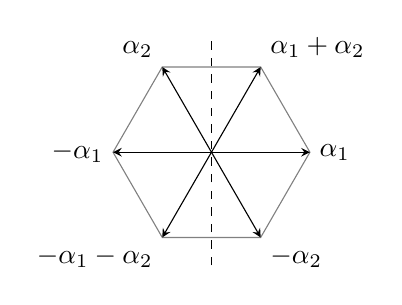
\begin{tikzpicture}[scale=1.25,>=stealth]
		\draw[gray] (0:1)--(60:1)--(120:1)--(180:1)--(240:1)--(300:1)--cycle;
		\draw[dashed] (0,-1.15)--(0,1.15);
		\foreach \a in {0,60,120,180,240,300} {\draw[->] (0,0)--(\a:1);}
		\node[right] at (0:1) {\(\symbfit\alpha_1\)};
		\node[above right] at (60:1) {\(\symbfit\alpha_1+\symbfit\alpha_2\)};
		\node[above left] at (120:1) {\(\symbfit\alpha_2\)};
		\node[left] at (180:1) {\(-\symbfit\alpha_1\)};
		\node[below left] at (240:1) {\(-\symbfit\alpha_1-\symbfit\alpha_2\)};
		\node[below right] at (300:1) {\(-\symbfit\alpha_2\)};
	\end{tikzpicture}
\]

% !TeX root = ../../Book5.tex
% 纲要标题：### 10.2 反射函子
% 纲要位置：工作记录/计划纲要.md，第 4058 行。
% * 汇点和源点反射
% * 对不可分解表示的作用
% * 与简单反射的对应
% * 从反射伴随的单位与余单位说明互逆范围，计算维数修正并区分子表示、商表示的封闭性
% * 明确汇点反射采用核、源点反射采用余核；给出排除相应简单表示后互为逆的范围，不把反射函子当作整个模范畴上的无条件等价
\section{反射函子}
\label{b5:sec:1002}

简单反射只改动一个整数坐标。在表示中实现这一运算，需要构造新的顶点空间，并相应改变邻接的箭映射。汇点上的核、源点上的余核给出所需构造。反射可能把一个简单表示消去，因此它不会给出整个表示范畴之间的等价。

\subsection{汇点反射与源点反射}
\label{b5:subsec:1002:01}

\begin{definition}\label{b5:def:reflection-functors}
	设 \(k\) 为域，\(Q\) 为有限无有向环箭图，\(i\) 为没有出箭的汇点，\(Q'\) 由反转所有以 \(i\) 为终点的箭得到。对 \(Q\) 的有限维 \(k\) 表示 \(V=(V_j,V_a)\)，令
	\[
		E_i(V)=\bigoplus_{a:j\to i}V_j,\qquad \phi_V:E_i(V)\longrightarrow V_i,\qquad (v_a)_a\longmapsto\sum_{a:j\to i}V_a(v_a).
	\]
	保留其他顶点空间，在 \(i\) 处取 \(\ker\phi_V\)；每条反转后的箭 \(a^*:i\to j\) 取包含映射 \(\ker\phi_V\hookrightarrow E_i(V)\) 与第 \(a\) 个投影的复合。所得 \(Q'\)-表示记为 \(F_i^+V\)，构造 \(F_i^+\) 称为\term{汇点反射函子}[sink reflection functor]。

	若 \(i\) 是没有入箭的源点，另令 \(Q'\) 为反转所有以 \(i\) 为起点的箭所得箭图，并令
	\[
		E_i(V)=\bigoplus_{a:i\to j}V_j,\qquad \psi_V:V_i\longrightarrow E_i(V),\qquad v\longmapsto\bigl(V_a(v)\bigr)_a.
	\]
	在 \(i\) 处取 \(\operatorname{coker}\psi_V\)，其他顶点不变；每条反转后的箭取相应直和包含与商映射的复合。所得表示记为 \(F_i^-V\)，构造 \(F_i^-\) 称为\term{源点反射函子}[source reflection functor]。
\end{definition}
\symidx{\(F_i^+,F_i^-\)：汇点与源点反射函子}

这里的直和以箭为指标。两条平行箭即使出自同一顶点，也对应两个独立的直和分量；漏掉这个重数会使维数公式错误。

\ProseParagraphBreak

还须说明这两个构造怎样作用于态射。若 \(f:V\to W\) 是表示态射，在汇点有
\[
	f_i\phi_V=\phi_W\left(\bigoplus_a f_{s(a)}\right).
\]
因此右侧直和映射把 \(\ker\phi_V\) 送入 \(\ker\phi_W\)，它的限制就是新顶点上的映射。各直和投影与此映射相容，保证反转后的箭图仍交换。在源点同样有
\[
	\left(\bigoplus_a f_{t(a)}\right)\psi_V=\psi_Wf_i,
\]
故直和映射诱导余核之间的映射；商映射与各直和包含相容。限制或取商都保持恒等态射、复合及态射的加法，所以确实得到两个加性 \(k\)-线性函子。汇点或源点反射不会制造有向圈，因为新箭图中的 \(i\) 分别成为源点或汇点，任何经过它的有向圈都不可能存在。

\subsection{反射函子对不可分解表示的作用}
\label{b5:subsec:1002:02}

记 \(S_i\) 为仅在顶点 \(i\) 处有一个 \(k\)、其余空间全为零的简单表示。以下分裂现象说明，反射唯一需要排除的不可分解对象正是 \(S_i\)。

\begin{lemma}\label{b5:lem:reflection-split-simple}
	设 \(k\) 为域，\(Q\) 为有限无有向环箭图，\(V=(V_j,V_a)\) 为有限维 \(k\) 表示，\(i\in Q_0\)。记 \(S_i\) 为只在顶点 \(i\) 取 \(k\) 的简单表示，\(\phi_V:\bigoplus_{a:j\to i}V_j\to V_i\) 为各入箭映射之和，\(\psi_V:V_i\to\bigoplus_{a:i\to j}V_j\) 为各出箭映射组成的映射，\(F_i^+,F_i^-\) 分别为汇点、源点反射函子。
	\begin{enumerate}
		\item 若 \(i\) 是汇点，则 \(\phi_V\) 满射当且仅当 \(V\) 没有非零的 \(S_i\) 直和项。
		\item 若 \(i\) 是源点，则 \(\psi_V\) 单射当且仅当 \(V\) 没有非零的 \(S_i\) 直和项。
	\end{enumerate}
	特别地，若 \(V\) 不可分解且 \(V\not\cong S_i\)，相应的满射或单射条件必成立；而 \(F_i^+S_i=0\) 或 \(F_i^-S_i=0\)。
\end{lemma}
\begin{proof}
	汇点情形取向量空间补空间 \(V_i=\operatorname{im}\phi_V\oplus U\)。所有进入 \(i\) 的箭都落在第一项，而 \(i\) 没有出箭。因此 \(V\) 分解为两个子表示：一个在 \(i\) 处取 \(\operatorname{im}\phi_V\)、其余顶点取原空间，另一个只在 \(i\) 处取 \(U\)。后一项同构于 \(S_i^{\oplus\dim U}\)。反过来，若存在这样的非零直和项，则入箭在该项上全为零，\(\phi_V\) 不可能满射。

	源点情形取 \(V_i=\ker\psi_V\oplus U\)。所有出箭在第一项上为零，且没有入箭，故只支撑于 \(\ker\psi_V\) 的部分是直和项；剩下的表示在 \(i\) 处取 \(U\)。存在非零 \(S_i\) 直和项也必使 \(\psi_V\) 有核。若 \(V\) 不可分解，分裂出的项只有在 \(V\cong S_i\) 时才可能非零。最后直接代入核或余核定义，\(S_i\) 均被送到零。
\end{proof}

源、汇条件保证分出的向量空间也是表示的直和项。在 \(1\to2\to3\) 的内部顶点 \(2\)，这一点已经会失败。区间表示 \(I[2,3]=(0\to k\xrightarrow{1}k)\) 的入箭总映射 \(0\to k\) 不满射，但 \(S_2\) 不是它的直和项：若把顶点 \(2\) 的 \(k\) 单独分出，出箭的恒等映射就不能保留。反过来，\(I[1,2]=(k\xrightarrow{1}k\to0)\) 的出箭总映射 \(k\to0\) 不单射，却也没有 \(S_2\) 直和项；顶点 \(2\) 的核虽给出子表示，非零入箭使它没有表示意义下的补项。这两个表示均不可分解，因为箭上的恒等映射迫使各非零顶点的自同态为同一个标量。

\subsection{反射函子与简单反射}
\label{b5:subsec:1002:03}

\begin{proposition}\label{b5:prop:reflection-dimension}
	设 \(k\) 为域，\(Q\) 为有限无有向环箭图，\(i\) 为汇点或源点，\(V=(V_j,V_a)\) 为有限维 \(k\) 表示。记 \(m_{ij}\) 为顶点 \(i,j\) 间的箭数，定义整数格变换 \((s_i\mathbf x)_i=-x_i+\sum_jm_{ij}x_j\)，其余坐标不变，此处不要求二次型正定。记 \(\phi_V:\bigoplus_{a:j\to i}V_j\to V_i\) 为各入箭映射之和、\(\psi_V:V_i\to\bigoplus_{a:i\to j}V_j\) 为各出箭映射组成的映射，\(\mathbf d\) 为维数向量，\(\mathbf e_i\) 为第 \(i\) 个坐标向量。若 \(i\) 为汇点，则
	\[
		\mathbf d(F_i^+V)=s_i\bigl(\mathbf d(V)\bigr) +\dim\operatorname{coker}\phi_V\,\mathbf e_i.
	\]
	若 \(i\) 为源点，则
	\[
		\mathbf d(F_i^-V)=s_i\bigl(\mathbf d(V)\bigr) +\dim\ker\psi_V\,\mathbf e_i.
	\]
	附加项的系数恰为 \(V\) 中可分出的 \(S_i\) 直和项的重数。因此汇点的 \(\phi_V\) 满射或源点的 \(\psi_V\) 单射时，维数向量按 \(s_i\) 变化。
\end{proposition}
\begin{proof}
	汇点处由秩与零度公式有
	\[
		\begin{aligned}
			\dim\ker\phi_V &=\sum_{a:j\to i}\dim V_j-\operatorname{rank}\phi_V\\
			&=\sum_{a:j\to i}\dim V_j-\dim V_i +\dim\operatorname{coker}\phi_V.
		\end{aligned}
	\]
	其他顶点维数不变，便得到第一式。源点处同样有
	\[
		\dim\operatorname{coker}\psi_V =\sum_{a:i\to j}\dim V_j-\dim V_i+\dim\ker\psi_V,
	\]
	得到第二式。\cref{b5:lem:reflection-split-simple}的构造在汇点分出 \(S_i^{\oplus\dim\operatorname{coker}\phi_V}\)，在源点分出 \(S_i^{\oplus\dim\ker\psi_V}\)，剩下的表示分别满足满射或单射条件。若另写成 \(V\cong S_i^{\oplus r}\oplus U\)，其中 \(U\) 不含 \(S_i\) 直和项，则分块总映射在 \(U\) 上满足相应条件，而在 \(S_i^{\oplus r}\) 上为零；故上述余核或核的维数必为 \(r\)。这也说明所计重数与补空间的选择无关。
\end{proof}

附加项不能省去。例如 \(1\to2\) 上的零箭表示 \(V=(k\xrightarrow{0}k)=S_1\oplus S_2\)，其汇点反射在顶点 \(2\) 取整个 \(k\)，所以 \(\mathbf d(F_2^+V)=(1,1)\)；而 \(s_2(1,1)=(1,0)\)，两者正好相差 \(\dim\operatorname{coker}(0:k\to k)\,\mathbf e_2=\mathbf e_2\)。特别是 \(s_i\mathbf e_i=-\mathbf e_i\)，反射函子却把 \(S_i\) 送到零；上述附加项补偿了这一差别。

\begin{example}\label{b5:exm:a3-sink-reflection}
	对 \(Q:1\to2\leftarrow3\)，取三个顶点空间均为 \(k\)，两条箭都为恒等映射。汇点 \(2\) 上的总映射是
	\[
		k\oplus k\longrightarrow k,\qquad (u,v)\longmapsto u+v.
	\]
	其核由 \((1,-1)\) 生成。反射后得到 \(1\leftarrow2\to3\)，两条箭分别由 \(1\) 与 \(-1\) 给出。新维数仍为 \((1,1,1)\)，与 \(s_2(1,1,1)=(1,1,1)\) 相符。改变顶点 \(3\) 的基可把第二条箭也变成 \(1\)；特征为 \(2\) 时它原先就等于 \(1\)。
\end{example}

\subsection{核、余核与反射函子的互逆范围}
\label{b5:subsec:1002:04}

\begin{proposition}[反射伴随]\label{b5:prop:reflection-adjunction}
	设 \(k\) 为域，\(Q\) 为有限无有向环箭图，\(i\) 为汇点，\(Q'\) 为反转 \(i\) 处各箭所得箭图。对任意有限维表示 \(W\in\operatorname{rep}_k Q'\)、\(V\in\operatorname{rep}_k Q\)，有自然的 \(k\)-线性同构
	\[
		\operatorname{Hom}_Q(F_i^-W,V) \cong\operatorname{Hom}_{Q'}(W,F_i^+V).
	\]
	即源点反射 \(F_i^-\) 是汇点反射 \(F_i^+\) 的左伴随，此处不要求排除简单直和项。记
	\[
		\phi_V:E_i(V)\longrightarrow V_i,\qquad \psi_W:W_i\longrightarrow E_i(W)
	\]
	为相应入箭之和与出箭组成的映射。单位与余单位为表示态射
	\[
		\eta_W:W\longrightarrow F_i^+F_i^-W,\qquad \varepsilon_V:F_i^-F_i^+V\longrightarrow V.
	\]
	两者在 \(i\) 以外的顶点均为恒等映射，在 \(i\) 处分别为
	\[
		\begin{aligned}
			(\eta_W)_i &: W_i\longrightarrow\operatorname{im}\psi_W, &w&\longmapsto\psi_W(w),\\
			(\varepsilon_V)_i &: E_i(V)/\ker\phi_V\longrightarrow V_i, &[x]&\longmapsto\phi_V(x).
		\end{aligned}
	\]
	其中 \((F_i^+F_i^-W)_i=\operatorname{im}\psi_W\)、\((F_i^-F_i^+V)_i=E_i(V)/\ker\phi_V\)。单位 \(\eta_W\) 总是满态射，且为同构当且仅当 \(\psi_W\) 单射；余单位 \(\varepsilon_V\) 总是单态射，且为同构当且仅当 \(\phi_V\) 满射。
\end{proposition}
\begin{proof}
	给定 \(i\) 以外的映射族 \(f_j:W_j\to V_j\)，先要求它与所有不接触 \(i\) 的箭相容。记各箭分量上的直和映射为 \(E(f):E_i(W)\to E_i(V)\)，并记商映射与包含映射为
	\[
		q_W:E_i(W)\longrightarrow E_i(W)/\operatorname{im}\psi_W, \qquad \kappa_V:\ker\phi_V\hookrightarrow E_i(V).
	\]
	将外部映射族延为 \(\alpha:F_i^-W\to V\)，须在 \(i\) 处找到 \(\alpha_i\)，使所有入箭交换。这些箭的直和包含合起来给出条件
	\[
		\alpha_iq_W=\phi_VE(f).
	\]
	因 \(q_W\) 满射，\(\alpha_i\) 至多有一个；它存在当且仅当
	\[
		\phi_VE(f)\psi_W=0.
	\]
	此时 \(\alpha_i\) 正是 \(\phi_VE(f)\) 在商空间上诱导的映射。另一方面，延为 \(\beta:W\to F_i^+V\) 所需的反向出箭交换条件，合起来是
	\[
		\kappa_V\beta_i=E(f)\psi_W.
	\]
	因 \(\kappa_V\) 单射，\(\beta_i\) 也至多有一个；它存在当且仅当同一个等式 \(\phi_VE(f)\psi_W=0\) 成立，此时由 \(E(f)\psi_W\) 限制值域得到。两边因而由相同的外部映射族描述，给出所述双射，并保持态射的加法与标量乘法。若分别在 \(W\)、\(V\) 两侧复合表示态射，外部直和映射随之复合，诱导的商映射与核映射也随之复合；故该同构对两个变量都自然。

	在上述对应中，\(\operatorname{id}_{F_i^-W}\) 对应的态射在 \(i\) 处由 \(\psi_W\) 限制值域到 \(\ker q_W=\operatorname{im}\psi_W\)，这就是 \(\eta_W\)。\(\operatorname{id}_{F_i^+V}\) 对应的态射在 \(i\) 处由 \(\phi_V\) 在 \(E_i(V)/\ker\phi_V\) 上诱导，这就是 \(\varepsilon_V\)。对每条 \(a:j\to i\)，\(\phi_V\) 与第 \(a\) 个包含的复合为 \(V_a\)；对每条 \(a^*:i\to j\)，\(\psi_W\) 与第 \(a\) 个投影的复合为 \(W_{a^*}\)。这具体说明两族顶点映射都与箭相容。

	若 \(h:V\to V'\)、\(g:W\to W'\) 为表示态射，则
	\[
		h_i\phi_V=\phi_{V'}E(h),\qquad E(g)\psi_W=\psi_{W'}g_i.
	\]
	取商或限制值域分别得到
	\[
		h\varepsilon_V=\varepsilon_{V'}F_i^-F_i^+(h),\qquad F_i^+F_i^-(g)\eta_W=\eta_{W'}g,
	\]
	因此余单位与单位都是自然变换。由这些公式直接复合，在顶点 \(i\) 分别得到 \(\ker\phi_V\) 与 \(E_i(W)/\operatorname{im}\psi_W\) 上的恒等映射，其他顶点也为恒等，故
	\[
		F_i^+(\varepsilon_V)\eta_{F_i^+V}=\operatorname{id}_{F_i^+V}, \qquad \varepsilon_{F_i^-W}F_i^-(\eta_W)=\operatorname{id}_{F_i^-W}.
	\]
	这也是单位、余单位的两个三角恒等式。最后，\(\psi_W:W_i\to\operatorname{im}\psi_W\) 满射，且其核为 \(\ker\psi_W\)；\(E_i(V)/\ker\phi_V\to V_i\) 单射，且其像为 \(\operatorname{im}\phi_V\)。其余顶点为恒等映射，所以单、满性及所述同构条件均成立。
\end{proof}

\begin{theorem}[反射等价]\label{b5:thm:reflection-equivalence}
	设 \(k\) 为域，\(Q\) 为有限无有向环箭图，\(i\) 为汇点，\(Q'\) 为反转 \(i\) 处各箭所得箭图。对有限维 \(k\) 表示 \(V\) 属于 \(Q\)、\(W\) 属于 \(Q'\)，分别记 \(\phi_V:\bigoplus_{a:j\to i}V_j\to V_i\) 为入箭映射之和，\(\psi_W:W_i\to\bigoplus_{a^*:i\to j}W_j\) 为出箭映射组成的映射。令 \(\mathcal C\) 为 \(\operatorname{rep}_k Q\) 中 \(\phi_V\) 满射的对象组成的全子范畴，\(\mathcal D\) 为 \(\operatorname{rep}_k Q'\) 中 \(\psi_W\) 单射的对象组成的全子范畴。则汇点反射函子和源点反射函子
	\[
		F_i^+:\mathcal C\longrightarrow\mathcal D,\qquad F_i^-:\mathcal D\longrightarrow\mathcal C
	\]
	互为拟逆。两边的对象条件分别等价于不含只在顶点 \(i\) 取 \(k\) 的简单表示 \(S_i\) 的非零直和项。
\end{theorem}
\begin{proof}
	对任意 \(V\)，\(F_i^+V\) 的源点总映射是包含 \(\ker\phi_V\hookrightarrow E_i(V)\)，所以它属于 \(\mathcal D\)。对任意 \(W\)，\(F_i^-W\) 的汇点总映射是商映射 \(E_i(W)\to E_i(W)/\operatorname{im}\psi_W\)，所以它属于 \(\mathcal C\)。由\cref{b5:prop:reflection-adjunction}，当 \(V\in\mathcal C\) 时，余单位 \(\varepsilon_V:F_i^-F_i^+V\to V\) 为同构；当 \(W\in\mathcal D\) 时，单位 \(\eta_W:W\to F_i^+F_i^-W\) 为同构。它们已经与各箭相容，并对态射自然，因而在这两个子范畴上给出所需的拟逆同构。两种对象条件的直和解释由\cref{b5:lem:reflection-split-simple}给出。
\end{proof}

\begin{corollary}\label{b5:cor:reflection-indecomposables}
	设 \(k\) 为域，\(Q\) 为有限无有向环箭图，\(i\) 为汇点或源点，\(Q'\) 为反转 \(i\) 处各箭所得箭图。以 \(S_i\) 分别表示两箭图中只在顶点 \(i\) 取 \(k\) 的简单表示，\(m_{ij}\) 为顶点 \(i,j\) 间的箭数，\((s_i\mathbf x)_i=-x_i+\sum_jm_{ij}x_j\)，其余坐标不变。相应汇点或源点反射函子，在 \(Q\) 与 \(Q'\) 中不同于 \(S_i\) 的不可分解有限维 \(k\) 表示的同构类之间给出双射，并保持它们的自同态代数；维数向量按 \(s_i\) 变化。
\end{corollary}
\begin{proof}
	这些不可分解对象都在\cref{b5:thm:reflection-equivalence}的相应全子范畴中。子范畴对直和项封闭：一个分块直和映射满射或单射，恰好当每个分块都如此。等价保持非零对象与直和分解，所以既保持也反映不可分解性；全忠实性给出自同态代数同构。维数变化由\cref{b5:prop:reflection-dimension}成立。
\end{proof}

上述全子范畴对直和项封闭，却不具有原表示范畴的全部子商封闭性。例如 \(1\to2\) 上的 \(P=(k\xrightarrow{1}k)\) 属于汇点 \(2\) 的 \(\mathcal C\)，但它的子表示 \(S_2=(0\to k)\) 不属于 \(\mathcal C\)。这一侧虽对商表示封闭，对任意子表示却不封闭。另一侧的 \(\mathcal D\) 对子表示封闭，因为单射 \(\psi_W\) 的限制仍单射；它对商表示不封闭：在 \(1\leftarrow2\) 上，\(P'=(k\xleftarrow{1}k)\) 属于 \(\mathcal D\)，商表示 \(P'/S_1=S_2\) 的源点总映射 \(k\to0\) 却不是单射。

\ProseParagraphBreak

在整个表示范畴上，汇点反射 \(F_i^+\) 是左正合函子，源点反射 \(F_i^-\) 是右正合函子。事实上，短正合列 \(0\to U\to V\to W\to0\) 在各顶点及各箭指标的直和上都保持正合。汇点总映射组成交换图，其核列
\[
	0\longrightarrow\ker\phi_U\longrightarrow\ker\phi_V \longrightarrow\ker\phi_W
\]
正合：若 \(\ker\phi_V\) 中的元素映到零，它在 \(E_i(U)\) 中有唯一原像；由 \(U_i\to V_i\) 单射，此原像仍落在 \(\ker\phi_U\)。源点总映射的余核列
\[
	\operatorname{coker}\psi_U\longrightarrow\operatorname{coker}\psi_V \longrightarrow\operatorname{coker}\psi_W\longrightarrow0
\]
正合：末项的每个类可由 \(E_i(V)\) 提升；若一个提升在 \(E_i(W)\) 中落入 \(\operatorname{im}\psi_W\)，先把相应的 \(W_i\) 元素提升到 \(V_i\)，减去其出箭像后便得到来自 \(E_i(U)\) 的代表元。其他顶点空间不变，故得到所述左、右正合性。

\ProseParagraphBreak

这两种函子一般不正合。对 \(1\to2\) 的短正合列
\[
	0\longrightarrow S_2\longrightarrow (k\xrightarrow{1}k)\longrightarrow S_1\longrightarrow0,
\]
取 \(F_2^+\) 后，中间项成为反向箭图上的 \(S_1\)，最后一项成为 \(P'=k\xleftarrow{1}k\)；诱导映射 \(S_1\to P'\) 在顶点 \(1\) 为恒等、顶点 \(2\) 为 \(0\to k\)，因而不是满态射。对反向箭图上的短正合列
\[
	0\longrightarrow S_1\longrightarrow P'=(k\xleftarrow{1}k)\longrightarrow S_2\longrightarrow0,
\]
取 \(F_2^-\) 后，前两项分别成为 \(P=(k\xrightarrow{1}k)\)、\(S_1\)，最后一项成为零；诱导映射 \(P\to S_1\) 在顶点 \(1\) 为恒等、顶点 \(2\) 为 \(k\to0\)，因而不是单态射。上述拟逆在排除相应简单直和项的全子范畴上成立；这两个短正合列显示，它们在整个表示范畴上分别失去了满射端与单射端的正合性。构造及其基本性质可参看\cite[Section 6.6, pp. 164--169]{EtingofEtAl2011RepresentationTheory}。

% !TeX root = ../../Book5.tex
% 纲要标题：### 10.3 Gabriel 定理
% 纲要位置：工作记录/计划纲要.md，第 4397 行。
% * 有限表示型与 Dynkin 图
% * 不可分解表示和正根
% * 无环及基域假设的明确版本
% * 分别证明有限表示型的必要性、Dynkin 情形的存在与唯一性，以及维数向量对正根的对应；定理固定有限箭图、无有向环、代数闭基域和有限维表示
% * 非连通箭图逐个连通分支处理：有限表示型对应 ADE 图的不交并，而非默认箭图连通
% * 用 A2 算例区分高度下降与汇点次序，以实数平均说明终止，并用两箭轨道方程解释参数计数
\section{Gabriel 定理}
\label{b5:sec:1003}

反射函子把相邻定向的表示联系起来，但任意挑选反射并不能保证分类过程终止。我们固定一个不断重复的汇点次序，证明在正定情形下，每个不可分解表示终会变成顶点简单表示。反过来，从简单表示沿原次序倒行，就能由正根构造出表示。

\subsection{有限表示型与 Dynkin 图}
\label{b5:subsec:1003:01}

\begin{definition}\label{b5:def:finite-quiver-type}
设 \(k\) 为域，\(Q\) 为有限箭图。若有限维不可分解 \(k\)-表示只有有限多个同构类，则称 \(Q\) 在 \(k\) 上具有\term{有限表示型}[finite representation type]；否则称为无限表示型。
\end{definition}

有限表示型不表示全部表示只有有限多个同构类。例如只有一个顶点且没有箭时，不可分解表示只有 \(k\) 这一个同构类；全部表示则按维数由 \(k^m\)（\(m\geq0\)）给出，彼此不同构，因此有无穷多个同构类。分类的对象是不能再作非平凡直和分解的部分。

\ProseParagraphBreak

接下来要证明两个不同方向的结论。正定型使反射过程终止，给出有限性及具体分类；非正定型则提供一个维数向量，使箭映射所含的自由参数多于换基能够消去的参数。后一论证不能由“二次型不是正定的”一句话代替。

\subsection{不可分解表示与正根}
\label{b5:subsec:1003:02}

对有限无有向环箭图，依次删去汇点，可以把顶点编号为 \(1,\ldots,n\)，使每条箭都从较大编号指向较小编号。先反射顶点 \(1\)，随后 \(2,\ldots,n\)：轮到 \(i\) 时，原先从 \(i\) 指向较小顶点的箭均已反转，而来自较大顶点的箭尚未反转，所以 \(i\) 确为当前箭图的汇点。一轮之后，每条箭的两端各反射一次，原方向恢复。

\ProseParagraphBreak

\cref{b5:lem:positive-root-reflection}中的高度下降，是在整数格中选择一个使正根坐标和减少的顶点；这个顶点未必是当前箭图的汇点。因此它不能直接保证上述固定次序的汇点反射会终止。要把反射实际施行于表示，必须遵守箭向，单步的坐标和也可能增加。

\begin{definition}\label{b5:def:quiver-coxeter-transformation}
设 \(Q\) 为有限无有向环箭图，将顶点编号为 \(1,\ldots,n\)，使每支箭都从较大编号指向较小编号。记 \(m_{ij}\) 为顶点 \(i,j\) 间的箭数，\(s_i\) 为整数格 \(\mathbb Z^{Q_0}\) 上的反射，其第 \(i\) 坐标为 \((s_i\mathbf x)_i=-x_i+\sum_jm_{ij}x_j\)，其余坐标不变。复合
\[
c=s_n s_{n-1}\cdots s_1
\]
称为这一编号下的\term{Coxeter 变换}[Coxeter transformation]。\footnote{考克斯特（Harold Scott MacDonald Coxeter，1907-2003），英裔加拿大数学家，研究反射群和多面体几何。}复合按从右到左作用，因此先施行 \(s_1\)。
\end{definition}
\symidx{\(c\)：编号确定的箭图 Coxeter 变换}

\begin{example}\label{b5:exm:a2-coxeter-sink-order}
设 \(k\) 为域，\(Q\) 为单箭图 \(2\to1\)，\(S_i\) 为仅在顶点 \(i\) 取 \(k\) 的简单表示。在顶点次序 \(1,2\) 下，整数格上的简单反射及一轮复合为
\[
s_1=\begin{pmatrix}-1&1\\0&1\end{pmatrix},\qquad
s_2=\begin{pmatrix}1&0\\1&-1\end{pmatrix},\qquad
c=s_2s_1=\begin{pmatrix}-1&1\\-1&0\end{pmatrix}.
\]
继续相乘得到
\[
c^2=\begin{pmatrix}0&-1\\1&-1\end{pmatrix},\qquad
c^3=I,\qquad I+c+c^2=0.
\]
从 \(S_2\) 出发，当前汇点是 \(1\)。入箭总映射为 \(k\to0\)，其核为 \(k\)；反转后的箭 \(1\to2\) 是恒等映射，故 \(F_1^+S_2\) 在两顶点均取 \(k\)。随后 \(2\) 成为汇点，其入箭映射为 \(1:k\to k\)，核为零，因此第二次反射得到原定向上的 \(S_1\)。维数向量依次为
\[
(0,1)\xrightarrow{s_1}(1,1)\xrightarrow{s_2}(1,0),
\]
坐标和先从 \(1\) 增至 \(2\)，再降至 \(1\)。虽然起点 \(S_2\) 已是简单表示，它却不是当前汇点 \(1\) 的简单表示，所以仍要继续反射；第二步之后，下一汇点为 \(1\)，才到达应当停止的 \(S_1\)。若再施行函子，则 \(F_1^+S_1=0\)，而整数格反射给出 \(s_1\mathbf e_1=-\mathbf e_1\)，两者的终点须加以区分。
\end{example}

\begin{lemma}\label{b5:lem:coxeter-exits-positive-cone}
设 \(Q\) 为有限无有向环箭图，将顶点编号为 \(1,\ldots,n\)，使每支箭都从较大编号指向较小编号。令 \(q_Q(\mathbf x)=\sum_i x_i^2-\sum_{a:i\to j}x_ix_j\) 为正定实二次型，\(B_Q(\mathbf x,\mathbf y)=q_Q(\mathbf x+\mathbf y)-q_Q(\mathbf x)-q_Q(\mathbf y)\)，\(\mathbf e_i\) 为标准基向量，\(s_i(\mathbf x)=\mathbf x-B_Q(\mathbf x,\mathbf e_i)\mathbf e_i\)，\(c=s_n\cdots s_1\)。则 \(c\) 有有限阶，\(1\) 不是其在 \(\mathbb R^{Q_0}\) 上的特征值，并且对每个非零非负实向量 \(\mathbf x\in\mathbb R^{Q_0}\)，存在整数 \(r\ge1\)，使 \(c^r\mathbf x\) 至少有一个负坐标。
\end{lemma}
\begin{proof}
由\cref{b5:thm:ade-positive-form}，基础图为 ADE 图的不交并。\cref{b5:lem:positive-root-reflection}说明各 \(s_i\) 保持有限的根集合，且标准基向量都是根。由这些反射生成的线性变换群在根集合上的作用是忠实的：固定全部根便固定一组基。因此它是有限置换群的子群，\(c^h=I\) 对某个正整数 \(h\) 成立。

若 \(c\mathbf x=\mathbf x\)，依次施行 \(s_1,\ldots,s_n\)。只有 \(s_i\) 能改变第 \(i\) 个坐标，而且之后的反射不会再次改变它。最终向量等于原向量，所以第一步没有改变坐标 \(1\)，即 \(s_1\mathbf x=\mathbf x\)；随后第二步也不改变坐标 \(2\)。逐步下去，所有 \(s_i\mathbf x=\mathbf x\)。由反射公式，\(B_Q(\mathbf x,\mathbf e_i)=0\) 对每个 \(i\) 成立，故正定性强迫 \(\mathbf x=0\)。这排除了特征值 \(1\)。

在实向量空间 \(\mathbb R^{Q_0}\) 上令
\[
T=I+c+\cdots+c^{h-1},\qquad P=\frac1h T.
\]
由 \(cT=T\)，\(P\) 的像包含在 \(c\) 的固定向量空间中；对每个固定向量 \(\mathbf y\)，又有 \(P\mathbf y=\mathbf y\)。所以 \(P\) 是到固定向量空间的投影。上一段已证明该空间为零，故 \(P=0\)，从而 \(T=0\)。若 \(\mathbf x\neq0\) 非负且所有 \(c^r\mathbf x\) 都非负，则
\[
0=T\mathbf x=\mathbf x+c\mathbf x+\cdots+c^{h-1}\mathbf x
\]
是包含一个非零项的非负向量之和，矛盾。
\end{proof}

有限阶本身并不能推出平均为零：在非零实向量空间上，恒等算子也有有限阶，却处处固定向量，其平均仍是恒等算子。上面的证明同时用了有限阶和没有非零固定向量这两个条件。平均是在将顶点整数格 \(\mathbb Z^{Q_0}\) 扩充为实向量空间 \(\mathbb R^{Q_0}\) 后计算，\(1/h\) 是实数标量，与表示的基域 \(k\) 的特征无关；若 \(\operatorname{char}k\) 整除 \(h\)，不能把 \(1/h\) 当作 \(k\) 中的标量。

\ProseParagraphBreak

正定条件失效时，非零非负向量可能始终不离开正锥。例如有两条平行箭 \(2\to1\) 的 Kronecker 箭图具有二次型 \(q_Q(x_1,x_2)=(x_1-x_2)^2\)。其坐标反射为
\[
s_1(x_1,x_2)=(-x_1+2x_2,x_2),\qquad
s_2(x_1,x_2)=(x_1,2x_1-x_2).
\]
非零非负向量 \(\symbfit\delta=(1,1)\) 被两者分别固定，因而也满足 \(c\symbfit\delta=\symbfit\delta\)。所以这里不能沿用 Coxeter 引理的正锥退出论证。

\ProseParagraphBreak

\cref{b5:lem:coxeter-exits-positive-cone}控制的是完整一轮反射。若从正根出发，在某一步第一次出现负坐标，则\cref{b5:lem:positive-root-reflection}说明前一步恰为当前顶点的简单根。因此，同一个终止论证既适用于表示的维数向量，也适用于尚未实现为表示的正根。此处采用的反射证明方法可对照\cite[Sections 6.7--6.8, pp. 169--172]{EtingofEtAl2011RepresentationTheory}。

\subsection{无环条件与基域假设}
\label{b5:subsec:1003:03}

本章分类定理固定代数闭域、有限无有向环箭图以及有限维表示，不附加箭之间的关系。无有向环条件保证汇点排序存在，也保证第九章使用的路径代数有限维。若加入关系，允许的箭矩阵不再遍历全部矩阵空间，下面的参数计数便不能原封不动地使用。

\ProseParagraphBreak

基域的作用也可以准确区分：核、余核、反射等价以及 Dynkin 情形的构造都只需要域公理；非 Dynkin 情形的参数论证需要域无限，代数闭域满足这一条件。有限域上一个固定维数向量只有有限多个矩阵组，所以不能照搬这个证明来推断存在无穷多个同维数类型。具体地，\(k=\mathbb F_q\) 上的 \(T^q-T\) 是非零多项式，却在 \(k\) 的每个元素处取零值；下面从多项式在全部点上取零值推出它为零的步骤，正是无限域假设的用途。我们不把当前证明未经核对地推广到更一般的基域情形。

\subsection{有限型的必要性、存在性与唯一性}
\label{b5:subsec:1003:04}

先看一个轨道能满足怎样的多项式方程。设 \(k\) 为无限域，\(Q\) 有两条平行箭 \(1\to2\)，在两顶点均取 \(k\)。箭映射由两个标量 \((a,b)\in k^2\) 给出，顶点换基 \((u,v)\in(k^\times)^2\) 把它们变为 \((va/u,vb/u)\)。因此非零矩阵组 \((a,b)\) 的轨道为
\[
\{\,t(a,b)\mid t\in k^\times\,\},
\]
它包含在非零多项式 \(bX-aY\) 的零点集中。零矩阵组的轨道只有 \((0,0)\)，也满足非零多项式方程 \(X=0\)。若只有有限多个轨道，将每个轨道的一个这样的多项式相乘，就会得到一个非零多项式，在全部 \(k^2\) 上取零值；无限域上这是不可能的。

\ProseParagraphBreak

在这个算例中，箭矩阵有两个自由参数，而换基只有比例 \(v/u\) 这一个有效参数。一般箭图上，换基含有矩阵逆，轨道因而由有理函数描述；下面用单项式个数的比较证明，只要箭参数多于有效换基参数，每个轨道仍满足某个非零多项式方程。这样就把必要性所需的参数计数写成可独立调用的引理。

\begin{lemma}\label{b5:lem:quiver-parameter-count}
设 \(k\) 为无限域，\(Q\) 为有限无有向环箭图，\(\mathbf d=(d_i)\in\mathbb Z_{\geq0}^{Q_0}\) 非零，\(q_Q(\mathbf d)=\sum_i d_i^2-\sum_{a:i\to j}d_id_j\)。若 \(q_Q(\mathbf d)\leq0\)，则维数向量为 \(\mathbf d\) 的有限维 \(k\)-表示有无穷多个同构类。
\end{lemma}
\begin{proof}
在每个顶点固定空间 \(k^{d_i}\)，所有箭映射组成仿射空间
\[
\operatorname{Rep}_k(Q,\mathbf d)
=\prod_{a:i\to j}M_{d_j\times d_i}(k)\cong k^N,\qquad
N=\sum_{a:i\to j}d_i d_j.
\]
换基群 \(G=\prod_{d_i>0}\operatorname{GL}_{d_i}(k)\) 的轨道恰好是同构类。记 \(m=\sum_i d_i^2\)，则假设给出 \(N\geq m\)。

固定一个表示矩阵组 \(A=(A_a)\)。轨道中的元素为
\[
\bigl(g_{t(a)}A_a g_{s(a)}^{-1}\bigr)_a.
\]
对所有 \(g_i\) 同时乘同一个非零标量不改变结果。选一个满足 \(d_{i_0}>0\) 的顶点；矩阵 \(g_{i_0}\) 的某个条目非零，可利用公共标量将它化为 \(1\)。固定这个非零条目的位置后，除它等于 \(1\) 以外，其余矩阵条目均可作为参数，共 \(m-1\) 个；公共标量已因不改变轨道元素而被消去。将这些条目代入轨道公式，矩阵求逆由代数余子式除以行列式给出，所以每个轨道坐标都是这些参数的有理函数，定义域要求各 \(\det g_i\ne0\)。非零条目的位置只有有限种选择，而每组换基矩阵都能作上述归一化。因此整个轨道被有限多个这样的有理映射的像覆盖，每个映射至多使用 \(m-1\) 个独立标量参数。

说明为何这样的像包含在某个非零多项式的零点集中。若 \(N\) 个有理函数 \(f_1,\ldots,f_N\) 只依赖 \(l<N\) 个变量，取非零共同分母 \(D\)，写 \(f_j=P_j/D\)。对指数向量 \(\mathbf e=(e_1,\ldots,e_N)\)、\(|\mathbf e|\le s\)，有
\[
D^s f_1^{e_1}\cdots f_N^{e_N}
=D^{s-|\mathbf e|}P_1^{e_1}\cdots P_N^{e_N}.
\]
取正整数 \(C\) 不小于 \(D,P_1,\ldots,P_N\) 的次数，右侧就是次数至多 \(Cs\) 的 \(l\) 元多项式。这些像共有 \(\binom{N+s}{N}\) 个，所在多项式空间的维数至多为 \(\binom{l+Cs}{l}\)。两数量关于 \(s\) 的增长次数分别为 \(N\) 和 \(l\)，且首项系数为正；因 \(N>l\)，充分大的 \(s\) 使前者更大。故存在不全为零的系数 \(c_{\mathbf e}\)，使 \(\sum_{|\mathbf e|\le s}c_{\mathbf e}D^sf^{\mathbf e}=0\)。多项式 \(P(Y_1,\ldots,Y_N)=\sum c_{\mathbf e}Y^{\mathbf e}\) 非零，因为不同 \(Y^{\mathbf e}\) 是形式单项式基；在有理函数域中消去非零的 \(D^s\)，便得 \(P(f_1,\ldots,f_N)=0\)。因此 \(P\) 在有理映射的定义域的像上为零。当前 \(l=m-1<N\)，所以每个参数片都具有这种关系；将有限多个关系相乘，得到在整个轨道上为零的非零多项式。

如果表示只有有限多个同构类，再把各轨道所得的多项式相乘，便得到在整个 \(k^N\) 上恒为零的非零多项式。这不可能：对无限域，非零一元多项式只有有限个根；对变量数归纳，把一个多元多项式视为最后一个变量的多项式，先使某个非零系数不消失，再选择最后一个变量，即能找到非零值。因此轨道有无穷多个。
\end{proof}

\begin{theorem}[Gabriel 定理]\label{b5:thm:gabriel}
设 \(k\) 为代数闭域，\(Q\) 为有限无有向环箭图，允许平行箭，表示均为没有额外关系的有限维 \(k\)-表示，\(q_Q(\mathbf x)=\sum_{i\in Q_0}x_i^2-\sum_{a:i\to j}x_ix_j\)。则 \(Q\) 具有有限表示型，当且仅当其无向基础图是 ADE 图的不交并。此时，维数向量给出双射
\[
\left\{\text{不可分解表示的同构类}\right\}
\longleftrightarrow
\bigl\{\symbfit\alpha\in\mathbb Z_{\geq0}^{Q_0}:
q_Q(\symbfit\alpha)=1\bigr\}.
\]
每个这样的不可分解表示 \(V\) 还满足
\(\operatorname{End}_Q(V)\cong k\) 及
\(\operatorname{Ext}^1_{kQ}(V,V)=0\)。
\end{theorem}
\begin{proof}
先证必要性。
若基础图不是 ADE 图的不交并，\cref{b5:thm:ade-positive-form}给出非零非负整数向量 \(\mathbf d\)，使 \(q_Q(\mathbf d)\leq0\)。代数闭域无限，故\cref{b5:lem:quiver-parameter-count}给出这一维数向量上的无穷多个同构类。

假设非零不可分解表示只有有限多个同构类型 \(U_1,\ldots,U_t\)，并记 \(D=\sum_i d_i\)。对任一维数向量为 \(\mathbf d\) 的表示，每次把一个可分解的非零直和项拆成两个非零项，非零直和项的数目增加 \(1\)；而每个非零项的总维数至少为 \(1\)，所以项数始终至多为 \(D\)。因此分裂过程在有限步后终止，所得各项均不可分解，从而该表示同构于
\[
U_1^{\oplus m_1}\oplus\cdots\oplus U_t^{\oplus m_t}.
\]
其中每个 \(m_j\) 都是满足 \(0\leq m_j\leq D\) 的整数。这样的整数元组只有有限多个，每个元组给出的直和也只有一个同构类型，故维数向量为 \(\mathbf d\) 的表示至多有有限多个同构类型，与参数计数引理矛盾。

现在基础图为 ADE 图的不交并，按汇点次序 \(1,\ldots,n\) 反复施行反射。从不可分解 \(V\neq0\) 出发，只要当前对象不同于所反射顶点的简单表示，\cref{b5:cor:reflection-indecomposables}就保证下一对象仍非零不可分解，维数向量按同一个简单反射变化。若过程永远不遇到该简单表示，每轮之后的维数向量便依次为
\(\mathbf d,c\mathbf d,c^2\mathbf d,\ldots\)，全部非负，与\cref{b5:lem:coxeter-exits-positive-cone}矛盾。因此某一步得到简单表示 \(S_i\)。简单反射保持 \(q_Q\)，故原维数向量满足 \(q_Q(\mathbf d)=q_Q(\mathbf e_i)=1\)，即为正根。

下面证明同一正根至多对应一个不可分解表示。
给定两个维数向量相同的不可分解表示，按相同的汇点次序反射。只要当前维数向量不是该顶点的 \(\mathbf e_i\)，两者都在相应反射等价的范围内。第一次达到 \(\mathbf e_i\) 时，两者都只能是 \(S_i\)。沿已经施行的等价逐步取拟逆，即得原来的两个表示同构。这个论证同时表明，停止时刻由维数向量确定，而不取决于箭映射的具体矩阵。

还需证明每个正根都能实现。
给定正根 \(\symbfit\alpha\)，按相同次序只在整数格中反射。由 Coxeter 引理，有限步后必首次出现负坐标。设这一负向量出现前的正根为 \(\symbfit\beta\)，下一步反射顶点为 \(i\)。由\cref{b5:lem:positive-root-reflection}，必有 \(\symbfit\beta=\mathbf e_i\)。在当时的定向上取 \(S_i\)，并按原次序的反序使用源点反射函子。

需要核实倒行过程不会把对象消去。由\cref{b5:lem:reflection-split-simple,b5:cor:reflection-indecomposables}，源点反射消去的不可分解对象只有该点的简单表示 \(S_j\)，其维数向量恰为 \(\mathbf e_j\)；其余不可分解对象仍非零不可分解。因此只需排查这种维数向量。若某一步要倒行经过顶点 \(j\)，而当前维数向量是 \(\mathbf e_j\)，则原正向过程在这一步之前的向量应为 \(s_j\mathbf e_j=-\mathbf e_j\)，与首次出现负向量以前各项均为正根矛盾。因此每个倒行步骤都避开被消去的简单表示，\cref{b5:cor:reflection-indecomposables}保证对象非零不可分解，并按原坐标序列恢复维数。最终得到维数向量为 \(\symbfit\alpha\) 的不可分解 \(Q\)-表示。

正根有限，所以双射也给出有限表示型。最后，每一步反射等价都保持自同态代数，而终点 \(S_i\) 的自同态代数为 \(k\)，故 \(\operatorname{End}_Q(V)\cong k\)。在\eqref{b5:eq:quiver-euler-hom-ext}中令 \(W=V\)，代入 \(q_Q(\mathbf d)=1\)，得到自扩张空间的维数为零。
\end{proof}

证明还给出了一个构造方法：输入 ADE 箭图的定向及一个正根，先记录汇点反射使它首次变负之前的全部步骤，再从末端的简单表示逐步取余核。每一步只需有限维线性代数。选择核、余核的不同基可能产生不同矩阵，但反射等价保证所得表示的同构类相同。

\ProseParagraphBreak

例如，把 \(D_4\) 的中心记为 \(0\)，三片叶记为 \(1,2,3\)，定向均为 \(i\to0\)。正根 \((2;1,1,1)\) 先在中心反射，再依次在三片叶反射，其维数变化为
\[
(2;1,1,1)\xrightarrow{s_0}(1;1,1,1)
\xrightarrow{s_1}(1;0,1,1)
\xrightarrow{s_2}(1;0,0,1)
\xrightarrow{s_3}(1;0,0,0).
\]
每次所反射的顶点都是当时的汇点。最后的简单表示在中心取 \(k\)。倒行时，先对叶 \(3,2,1\) 作源点反射：各次余核都是 \(\operatorname{coker}(0\to k)=k\)，所以得到中心向三片叶的恒等映射。再在中心取余核，得到
\[
k\xrightarrow{z\mapsto(z,z,z)}k^3
\longrightarrow k^3/k(1,1,1).
\]
原定向的三支箭分别把 \(1\) 送到坐标向量的商类 \(\bar e_1,\bar e_2,\bar e_3\)。其中前两类构成一组基，而 \(\bar e_3=-\bar e_1-\bar e_2\)；把第三片叶的基乘以 \(-1\)，便得到三支箭的列向量 \((1,0)^{\mathsf T},(0,1)^{\mathsf T},(1,1)^{\mathsf T}\)。这就从简单表示实际构造出中心二维、三片叶一维的不可分解表示，特征为二时同样成立。

\subsection{非连通箭图与 ADE 图的不交并}
\label{b5:subsec:1003:05}

若 \(Q\) 的连通分支为 \(Q^{(1)},\ldots,Q^{(r)}\)，任何表示都按支集唯一分成各分支上的表示的直和。因而非零不可分解表示只支撑在一个分支上。二次型也按分支相加；在正定情形，整数向量的每个非零分支至少贡献 \(1\)，所以正根同样只支撑在一个分支上。Gabriel 对应在这里逐分支进行，不需要给非连通图强加一个连通的 Dynkin 名称。

\begin{example}\label{b5:exm:an-positive-roots}
设 \(k\) 为域，\(n\geq1\)，\(Q\) 为链 \(A_n\) 的任意定向，顶点沿链标为 \(1,\ldots,n\)。令 \(q(\mathbf x)=\sum_{i=1}^n x_i^2-\sum_{i=1}^{n-1}x_ix_{i+1}\)，以 \(q=1\) 的非负整数向量为正根。补记 \(x_0=x_{n+1}=0\)，则
\[
2q(\mathbf x)=\sum_{i=0}^{n}(x_{i+1}-x_i)^2.
\]
若 \(\mathbf x\) 是整数正根，右侧等于 \(2\)。全部整数差中只能有两个非零项，各自为 \(1\) 或 \(-1\)；它们的和为零，所以必为一个 \(1\) 和一个 \(-1\)。非负性又要求先出现 \(1\)。因此正根恰为某段连续顶点上全为 \(1\)、其余为零的向量，共有 \(n(n+1)/2\) 个。任意定向下，在这段顶点取 \(k\)，内部各箭取恒等映射，外部空间取零，就得到相应的不可分解表示：所有非零顶点上的自同态标量因箭交换条件而相等，所以自同态代数为 \(k\)，不可能存在非平凡直和分解所产生的幂等元。
\end{example}

例如 \(A_2\) 与 \(A_1\) 的不交并有 \(3+1=4\) 个不可分解类型，而不是 \(3\cdot1\) 个。直和组合描述全部表示，分支的并则描述不可分解类型；两种计数的对象不同。

% !TeX root = ../../Book5.tex
% 纲要标题：### 10.4 表示型与几乎分裂序列
% 纲要位置：工作记录/计划纲要.md，第 4406 行。
% * Kronecker 箭图
% * 驯型、野型与三箭图
% * Auslander–Reiten 理论的基本问题
% ---
\section{表示型与几乎分裂序列}
\label{b5:sec:1004}

ADE 图给出有限分类，图稍有扩大就可能出现带参数的不可分解表示。不过，“出现参数”并不等于“分类已无法描述”。本节用两条平行箭和三条平行箭比较两种不同的复杂程度，再用一个最小例子说明 Auslander--Reiten 理论\footnote{奥斯兰德（Maurice Auslander，1926-1994），美国数学家，研究同调代数与表示论；赖滕（Idun Reiten，1942-2025），挪威数学家，研究有限维代数的表示与倾斜理论。}研究什么。

\subsection{Kronecker 箭图}
\label{b5:subsec:1004:01}

\begin{definition}\label{b5:def:kronecker-quiver}
	有两个顶点 \(1,2\)，以及两条从 \(1\) 指向 \(2\) 的平行箭的箭图，称为\term{Kronecker 箭图}[Kronecker quiver]。\footnote{克罗内克（Leopold Kronecker，1823-1891），德国数学家，研究代数数论与代数方程。}给定域 \(k\)，它的一个有限维 \(k\)-表示是一对有限维 \(k\) 向量空间之间具有相同定义域和值域的线性映射
	\[
		A,B:V_1\longrightarrow V_2.
	\]
	同构是同时作用于两条映射的定义域换基和值域换基。
\end{definition}

它的二次型为 \(q(d_1,d_2)=(d_1-d_2)^2\)，所以并不正定。对每个 \(\lambda\in k\)，取两端空间为 \(k\)，箭为 \(1,\lambda\)，记所得表示为 \(R_\lambda\)。若两端换基标量为 \(a,b\)，第一条箭的交换条件给出 \(a=b\)，第二条箭随即给出 \(\lambda=\mu\)。故 \(R_\lambda\cong R_\mu\) 当且仅当 \(\lambda=\mu\)。每个 \(R_\lambda\) 的自同态代数为 \(k\)，所以不可分解；另有两箭为 \(0,1\) 的 \(R_\infty\)，它与前述各项不同构。

任意维数向量为 \((1,1)\) 的表示都由一个箭对 \((a,b)\in k^2\) 给出，两端换基只把它乘以一个共同的非零标量。当 \((a,b)\ne(0,0)\) 时，同构参数便是比例 \([a:b]\)，即射影直线 \(\mathbb P^1(k)\) 的点。\(a\ne0\) 的参数可写成 \([1:\lambda]\)，对应 \(R_\lambda\)；剩余的 \([0:1]\) 对应 \(R_\infty\)。原点则对应可分解表示 \(S_1\oplus S_2\)。

这些参数未必能由整个表示空间上的多项式不变量区分。以 \(k=\mathbb C\) 为例，换基的有效作用是 \(\mathbb C^\times\) 对 \(\mathbb C^2\) 的共同缩放。若多项式 \(F(a,b)\) 不变，把它分为各次齐次分量；次数为 \(d\) 的分量在缩放 \((a,b)\mapsto(za,zb)\) 下乘以 \(z^d\)。对所有 \(z\ne0\) 比较 \(F(za,zb)=F(a,b)\) 中的 \(z\) 次幂，正次数分量只能为零。因此
\[
	\mathbb C[a,b]^{\mathbb C^\times}=\mathbb C.
\]
每个非零轨道的闭包都含原点，所以多项式不变量把所有这些轨道与原点送到同一个值。另一方面，每个非零箭对都给出非分裂扩张 \(0\to S_2\to R\to S_1\to0\)，其合成因子与原点相同，都是 \(S_1,S_2\)，而比例 \([a:b]\) 记录这两个因子之间的作用关系。故分类同构类型的参数与多项式不变量商不能混同；\subsecref{b5:subsec:2206:01}将建立仿射商的泛性质，\subsecref{b5:subsec:2206:03}再用此处的 Kronecker 参数例子说明这个区别。

\begin{proposition}\label{b5:prop:kronecker-jordan-family}
	设 \(k\) 为代数闭域，\(Q\) 为两支箭均由顶点 \(1\) 指向顶点 \(2\) 的 Kronecker 箭图，\(r\geq1\) 为整数，\(\lambda\in k\)，\(J_r(\lambda)\) 为大小 \(r\) 的 Jordan 块。两顶点空间均取 \(k^r\)，则箭映射给出的表示
	\[
		R_{\lambda,r}=\bigl(I_r,J_r(\lambda)\bigr),\qquad R_{\infty,r}=\bigl(J_r(0),I_r\bigr)
	\]
	均不可分解。对固定 \(r\)，它们由 \(\lambda\in k\cup\{\infty\}\) 给出两两不同的同构类，而且
	\[
		\dim_k\operatorname{End}_Q(R_{\lambda,r}) =\dim_k\operatorname{Ext}^1_{kQ}(R_{\lambda,r},R_{\lambda,r})=r,
	\]
	其中也允许 \(\lambda=\infty\)。
\end{proposition}
\begin{proof}
	对有限 \(\lambda\)，第一条箭为恒等，故自同态的两端矩阵相同，并与 \(J_r(\lambda)\) 对易。令 \(N=J_r(\lambda)-\lambda I_r\)。Jordan 块有循环向量 \(v\)，使 \(v,Nv,\ldots,N^{r-1}v\) 为一组基。与 \(N\) 对易的算子由 \(v\) 的像唯一决定；若其像为 \(\sum_{j=0}^{r-1}a_jN^jv\)，该算子便是 \(\sum_j a_jN^j\)。因此
	\[
		\operatorname{End}_Q(R_{\lambda,r})\cong k[t]/(t^r).
	\]
	这个环的每个元素若常数项非零就可逆，若常数项为零则幂零，所以幂等元只有 \(0,1\)。非平凡直和分解会给出非平凡投影幂等元，故表示不可分解。无穷参数的情形只需用第二条恒等箭，计算相同。

	两个有限参数表示的同构要求两个 Jordan 块相似，因而由唯一特征值分别为 \(\lambda,\mu\) 得 \(\lambda=\mu\)。无穷参数中第一条箭不可逆，而有限参数中第一条箭可逆，所以它们不同构。最后，自同态维数为 \(r\)，而 \(q(r,r)=0\)，由\eqref{b5:eq:quiver-euler-hom-ext}得到自扩张维数也为 \(r\)。
\end{proof}

上式给出的族并未穷尽全部不可分解表示。例如维数向量 \((1,2)\)、两箭分别取 \(1\mapsto(1,0)\) 与 \(1\mapsto(0,1)\) 的表示，其自同态也只有标量，却不属于维数为 \((r,r)\) 的那些族。完整分类还要处理维数不同的两端及一般矩阵铅笔；可把这一问题作为后续专题，参看\cite[Problem 6.9.1(d), p. 174]{EtingofEtAl2011RepresentationTheory}。

\subsection{驯型、野型与三箭图}
\label{b5:subsec:1004:02}

为了区分“由少量参数族描述”和“包含任意矩阵对的分类”，先给出常用的精确定义。以下只讨论代数闭域上的有限维代数；路径代数 \(kQ\) 在有限无有向环条件下属于这个范围。

\begin{definition}\label{b5:def:tame-wild-type}
	设 \(k\) 为代数闭域，\(A\) 为有限维含幺 \(k\)-代数。
	\begin{enumerate}
		\item 若 \(A\) 有无限多个有限维不可分解左模的同构类，且对每个整数 \(d\geq1\)，存在有限多个 \(A\)-\(k[t]\) 双模 \(M_1,\ldots,M_s\)，每个作为右 \(k[t]\)-模自由且秩为 \(d\)，使除有限多个例外外，每个 \(d\) 维不可分解左 \(A\)-模都同构于某个
			\[
				M_j\otimes_{k[t]}k[t]/(t-\lambda)\qquad(\lambda\in k),
			\]
			则称 \(A\) 具有\term{驯表示型}[tame representation type]。
		\item 令 \(R=k\langle x,y\rangle\) 为两个非交换变量上的自由结合代数。若存在 \(A\)-\(R\) 双模 \(M\)，作为右 \(R\)-模自由且有限秩，使函子
			\[
				M\otimes_R-:\{\text{有限维左 }R\text{-模}\} \longrightarrow\{\text{有限维左 }A\text{-模}\}
			\]
			保持不可分解性，并且两个输入的像同构当且仅当输入本身同构，则称 \(A\) 具有\term{野表示型}[wild representation type]。
	\end{enumerate}
\end{definition}

驯型定义要求在每个维数上穷尽几乎所有不可分解类型，而不是仅仅找到几个单参数族。上一小节的 Jordan 族本身还不足以证明 Kronecker 箭图为驯型。野型定义中的右自由条件保证张量函子正合；它所嵌入的 \(R\)-模分类恰好是任意两个方阵在同时相似下的分类，因为 \(x,y\) 可以独立作用为任意两个算子。

\ProseParagraphBreak

驯型定义中的右自由条件也有具体作用。对秩为 \(d\) 的双模 \(M\) 选一组右 \(k[t]\)-基，左 \(A\) 作用因与右作用交换而给出代数同态 \(A\to\operatorname{End}_{k[t]}(M)\cong M_d(k[t])\)。把矩阵条目中的 \(t\) 代成 \(\lambda\)，就得到 \(M\otimes_{k[t]}k[t]/(t-\lambda)\) 上的作用矩阵。右自由性保证这一空间对每个 \(\lambda\) 都为 \(k^d\)，因此这是维数固定的多项式矩阵族；若仅有一个任意有限生成右模，特殊参数处的维数可能改变。

\begin{proposition}\label{b5:prop:three-kronecker-wild}
	设 \(k\) 为代数闭域，\(Q\) 为具有两顶点及三条从 \(1\) 指向 \(2\) 的平行箭的箭图。则 \(kQ\) 为野表示型。
\end{proposition}
\begin{proof}
	将一个有限维 \(R=k\langle x,y\rangle\)-模写为 \((V,X,Y)\)，其中 \(X,Y\) 是 \(x,y\) 的作用。给它对应 \(Q\)-表示
	\[
		F(V,X,Y)=(V,V;I_V,X,Y).
	\]
	两端映射 \((f_1,f_2)\) 对第一条箭的相容条件为 \(f_2I_V=I_{V'}f_1\)，强迫 \(f_1=f_2=f\)；余下条件恰好为 \(fX=X'f\)、\(fY=Y'f\)。所以 \(F\) 在态射上给出双射，特别是保持自同态代数并反映同构。一个表示可分解当且仅当其自同态代数有非平凡幂等元：投影给出一个方向，另一个方向由幂等元的像与核给出。因此 \(F\) 保持不可分解性。

	最后核实双模条件。取顶点 \(1,2\) 上都为右 \(R\)-模 \(R\)，三条箭分别为恒等映射、左乘 \(x\)、左乘 \(y\)。它们是右 \(R\)-线性映射，故组成一个 \(kQ\)-\(R\) 双模 \(M\)。其右 \(R\)-模为 \(R\oplus R\)，自由秩为 \(2\)。经两个顶点上的自然同构 \(R\otimes_R V\cong V\)，\(M\otimes_R V\) 识别为上述 \(F(V,X,Y)\)。对任意 \(R\)-模同态 \(f:V\to V'\)，\(1_M\otimes f\) 在两个顶点上都识别为 \(f\)，与 \(F(f)=(f,f)\) 一致。因此 \(M\otimes_R-\cong F\) 是函子层面的自然同构，满足野型定义。
\end{proof}

上述例子给出三种情形：ADE 箭图只有有限多个不可分解类型，Kronecker 箭图出现显式单参数族，三箭图包含任意矩阵对的同时相似问题。把一般有限维代数的无限型进一步分为驯型与野型，还需要更深入的分类理论。

\subsection{Auslander--Reiten 理论的基本问题}
\label{b5:subsec:1004:03}

Gabriel 定理列出了对象，却没有列出对象之间的全部态射。Auslander--Reiten 理论进一步研究：哪些非分裂态射能够控制其他态射的分解，哪些短正合列能够系统地组织不可分解对象之间的联系。

\begin{definition}\label{b5:def:almost-split-sequence}
	设 \(k\) 为域，\(A\) 为有限维含幺 \(k\)-代数，\(X,E,Z\) 为有限维左 \(A\)-模，\(p:E\to Z\) 为模同态。若 \(p\) 不是分裂满射，且对每个有限维左 \(A\)-模 \(Y\) 及每个不是分裂满射的模同态 \(f:Y\to Z\)，存在模同态 \(h:Y\to E\) 使 \(f=ph\)，则称 \(p\) 为\term{右几乎分裂态射}[right almost split morphism]。对偶地，给定模同态 \(u:X\to E\)，若 \(u\) 不是分裂单射，且每个不是分裂单射的模同态 \(g:X\to Y\) 都经 \(u\) 分解，则称 \(u\) 为\term{左几乎分裂态射}[left almost split morphism]。一个非分裂短正合列
	\[
		0\longrightarrow X\xrightarrow{u}E\xrightarrow{p}Z\longrightarrow0
	\]
	若两端 \(X,Z\) 非零不可分解，且 \(u,p\) 分别具有上述左、右性质，则称为\term{几乎分裂序列}[almost split sequence]，也称 Auslander--Reiten 序列。\termidx{Auslander--Reiten 序列}
\end{definition}

这些定义中的“分裂”是范畴中的分裂，要求左逆或右逆本身也是模同态；向量空间上的任意补空间不够。

\begin{example}\label{b5:exm:a2-almost-split}
	对任意域 \(k\) 及箭图 \(Q:1\to2\)，有几乎分裂序列
	\[
		0\longrightarrow S_2\longrightarrow P\longrightarrow S_1\longrightarrow0,\qquad P=(k\xrightarrow{1}k).
	\]
	其中左映射在顶点 \(2\) 为恒等，右映射在顶点 \(1\) 为恒等。
\end{example}
\begin{proof}
	序列逐顶点正合。若它分裂，则 \(P\cong S_1\oplus S_2\)，而后者箭映射为零，与 \(P\) 的箭映射秩为 \(1\) 矛盾。

	设 \(Y=(Y_1\xrightarrow{T}Y_2)\)。态射 \(f:Y\to S_1\) 由任意线性泛函 \(f_1:Y_1\to k\) 给出。它是分裂满射，当且仅当有 \(v\in\ker T\) 使 \(f_1(v)=1\)：这样的 \(v\) 正好定义一个右逆 \(S_1\to Y\)。因此若 \(f\) 不是分裂满射，\(f_1\) 必在 \(\ker T\) 上为零。它于是经 \(T\) 的像分解为泛函，并可延拓为 \(h_2:Y_2\to k\)，满足 \(h_2T=f_1\)。两端取 \(h_1=f_1,h_2\)，得到态射 \(h:Y\to P\)，并有 \(f=ph\)。这证明右几乎分裂性质。

	态射 \(g:S_2\to Y\) 由一个向量 \(w\in Y_2\) 给出。它有左逆，当且仅当存在泛函 \(\ell:Y_2\to k\)，满足 \(\ell T=0\)、\(\ell(w)=1\)，也就是 \(w\notin\operatorname{im}T\)。因此若 \(g\) 不是分裂单射，必有 \(w=T(v)\) 对某个 \(v\in Y_1\) 成立。把 \(1\in P_1\) 送到 \(v\)、把 \(1\in P_2\) 送到 \(w\)，就得到态射 \(P\to Y\)，使 \(g\) 经左映射分解。这证明左几乎分裂性质。两端简单表示当然不可分解。
\end{proof}

在一般理论中，人们把几乎分裂序列左端的同构类记作 \(\tau Z\)，并研究这些序列的存在、唯一性及中间项的不可分解成分；本章只讨论了上面的例子。当前例子说明 \(\tau S_1\cong S_2\)，这里的 \(\tau\) 记录几乎分裂序列的左端同构类；这个说法没有在全体模范畴上定义一个自同构函子。特别是，若终点 \(Z\) 为投射模，任何以它为终点的短正合列都分裂，因此不存在这种非分裂序列。对象分类与态射结构在这里成为两个互相补充的问题。

% !TeX root = ../../Book5.tex
% 纲要标题：### 10.5 不可约映射与几乎分裂序列
% 纲要位置：工作记录/计划纲要.md（2026-10-20 新增骨架）。
% 写作状态：2026-10-20 新增骨架；正文、证明、算例与习题均待撰写。
% 写作范围：Krull–Schmidt 及局部自同态环引用第二卷第12章；承接第10.4节的定义与 A2 算例，不重建已有理论。
% #### 10.5.1 态射根与不可约映射
% #### 10.5.2 极小几乎分裂态射
% #### 10.5.3 几乎分裂序列的存在与唯一性

\section{不可约映射与几乎分裂序列}
\label{b5:sec:1005}

待撰写。

\subsection{态射根与不可约映射}
\label{b5:subsec:1005:01}

待撰写。

\subsection{极小几乎分裂态射}
\label{b5:subsec:1005:02}

待撰写。

\subsection{几乎分裂序列的存在与唯一性}
\label{b5:subsec:1005:03}

待撰写。

% 新增结构与纲要同步；以下条目均为待撰写计划。
% * 状态：待撰写；当前仅有结构占位。

% !TeX root = ../../Book5.tex
% 纲要标题：### 10.6 AR 平移与公式
% 纲要位置：工作记录/计划纲要.md（2026-10-20 新增骨架）。
% 写作状态：2026-10-20 新增骨架；正文、证明、算例与习题均待撰写。
% 写作范围：固定有限维左模及 DTr 的侧别，区分稳定与余稳定 Hom；不把 AR 平移当作整个模范畴上的自等价。
% #### 10.6.1 转置模、对偶与 AR 平移
% #### 10.6.2 稳定与余稳定范畴
% #### 10.6.3 Auslander–Reiten 公式及其适用条件

\section{AR 平移与公式}
\label{b5:sec:1006}

待撰写。

\subsection{转置模、对偶与 AR 平移}
\label{b5:subsec:1006:01}

待撰写。

\subsection{稳定与余稳定范畴}
\label{b5:subsec:1006:02}

待撰写。

\subsection{Auslander–Reiten 公式及其适用条件}
\label{b5:subsec:1006:03}

待撰写。

% 新增结构与纲要同步；以下条目均为待撰写计划。
% * 状态：待撰写；当前仅有结构占位。

% !TeX root = ../../Book5.tex
% 纲要标题：### 10.7 AR 箭图与表示型
% 纲要位置：工作记录/计划纲要.md（2026-10-20 新增骨架）。
% 写作状态：2026-10-20 新增骨架；正文、证明、算例与习题均待撰写。
% 写作范围：计算 An 型及 Kronecker 的预投射、正则和预内射分支；仿射箭图和 Drozd 定理固定适用范围，不重建已有 Tits 型。
% #### 10.7.1 线性定向箭图的 AR 箭图
% #### 10.7.2 Kronecker 箭图的三个分支
% #### 10.7.3 仿射箭图与表示型
% #### 10.7.4 驯野二分定理的陈述

\section{AR 箭图与表示型}
\label{b5:sec:1007}

待撰写。

\subsection{线性定向箭图的 AR 箭图}
\label{b5:subsec:1007:01}

待撰写。

\subsection{Kronecker 箭图的三个分支}
\label{b5:subsec:1007:02}

待撰写。

\subsection{仿射箭图与表示型}
\label{b5:subsec:1007:03}

待撰写。

\subsection{驯野二分定理的陈述}
\label{b5:subsec:1007:04}

待撰写。

% 新增结构与纲要同步；以下条目均为待撰写计划。
% * 状态：待撰写；当前仅有结构占位。
% ---


\begin{chaptersummary}
	Euler 型由顶点和箭的数值资料定义，却等于 Hom 与 Ext 的维数差。正定判别不依赖表示的箭矩阵：重边、圈、四叉及双三叉都会给出一个非零非负整数向量 \(\mathbf d\)，使 \(q_Q(\mathbf d)\leq0\)，剩下的三臂树由倒数和不等式筛选出 ADE 图。正定整数格中的根与简单反射因而可以在学习 Lie 代数以前建立。

	\ProseParagraphBreak

	反射函子把整数格的运算实现为核或余核。在排除相应顶点简单直和项的全子范畴上，它们互为拟逆；对不可分解对象，这正好排除唯一可能被消去的简单表示。Coxeter 变换控制重复反射的终止，由此证明每个 Dynkin 不可分解表示都来自一个简单表示，也证明每个正根能沿逆过程唯一实现。非正定情形的必要性则依赖参数计数：在代数闭域上，对所构造的非零维数向量 \(\mathbf d\)，记 \(m=\sum_i d_i^2\)。公共标量的作用为恒等，使每个换基轨道至多具有 \(m-1\) 个独立参数，而表示矩阵空间有 \(\sum_{a:i\to j}d_id_j\ge m\) 个参数，因而不能只有有限多个轨道。

	\ProseParagraphBreak

	不可约映射由态射根模去根平方刻画，极小右几乎分裂映射的分量给出终到一个不可分解模的全部不可约箭。极小投射展示构造的 \(\tau=D\operatorname{Tr}\) 在稳定与余稳定范畴之间给出等价；AR 对偶再从自同态环的剩余除代数中选取泛函，构造几乎分裂序列。一般公式中的稳定商不可省略，无关系无环路径代数的遗传性才给出相应的普通 Hom 公式。

	\ProseParagraphBreak

	线性定向的 \(A_n\) 由区间端点给出有限的 AR 箭图。Kronecker 标准形将不可分解表示分为预投射、预内射和正则三类；显式同态计算给出各类的几乎分裂序列，正则部分形成按射影直线参数化的齐性管。仿射箭图仍属驯型，但正则部分可以出现更高周期的管。Kronecker 标准形的穷尽性、一般仿射分类与 Drozd 二分在本章给出证明概要，具体序列的正合性与因子分解则逐一证明。表示型的判定既要控制所有维数，也要证明参数族穷尽或构造表示嵌入，不能由少量算例替代。
\end{chaptersummary}

\BookExercises

\begin{optionalexercise}\label{b5:ex:10-euler-orientation}
	设 \(Q:1\to2\leftarrow3\)。写出满足 \(\langle\mathbf x,\mathbf y\rangle_Q=\mathbf x^{\mathsf T}E\mathbf y\) 的矩阵 \(E\)，并计算 \(q_Q(2,1,1)\)。反转箭 \(1\to2\) 后，指出 \(E\) 哪些条目改变，并说明二次型为何不变。
\end{optionalexercise}
\begin{solution}
	由两条箭的贡献，
	\[
		E=\begin{pmatrix}1&-1&0\\0&1&0\\0&-1&1\end{pmatrix},
		\qquad q_Q(2,1,1)=4+1+1-2-1=3.
	\]
	反转第一条箭使 \(E_{12}\) 由 \(-1\) 变成 \(0\)，\(E_{21}\) 由 \(0\) 变成 \(-1\)，其余不变。二次型原来的项 \(-x_1x_2\) 变成 \(-x_2x_1\)，故数值完全相同；非对称的 Euler 型则已经改变。
\end{solution}

\begin{optionalexercise}\label{b5:ex:10-hom-orientation}
	对 \(Q:1\to2\)，记 \(P=(k\xrightarrow{1}k)\)。计算 \(\operatorname{Hom}_Q(S_1,P)\)、\(\operatorname{Hom}_Q(P,S_1)\) 及对应的两个 \(\operatorname{Ext}^1\)。将箭反转，对相同维数向量的表示重复 Hom 计算。
\end{optionalexercise}
\begin{solution}
	态射 \(S_1\to P\) 的顶点 \(1\) 映射被箭交换条件迫为零，故 Hom 为零；态射 \(P\to S_1\) 的顶点 \(1\) 映射可以是任意标量，故 Hom 同构于 \(k\)。Euler 数分别为 \(\bigl\langle(1,0),(1,1)\bigr\rangle_Q=0\)、 \(\bigl\langle(1,1),(1,0)\bigr\rangle_Q=1\)，所以两个 Ext 都为零。 反向箭图的 \(P'=(k\xleftarrow{1}k)\) 满足 \(\operatorname{Hom}(S_1,P')\cong k\)、 \(\operatorname{Hom}(P',S_1)=0\)。 根集合不依赖定向，但根所标记对象之间的态射空间会随定向改变。
\end{solution}

\begin{optionalexercise}\label{b5:ex:10-affine-three-arm}
	设树有一个三叉点，三个臂长为 \(1,2,5\)。构造一个所有坐标为正的整数向量，使二次型为零；再说明把最长臂末端删去后为什么变成正定型。
\end{optionalexercise}
\begin{solution}
	三个参数为 \(p=2,q=3,r=6\)，其倒数之和为 \(1\)。中心取 \(6\)，三个臂从中心向外分别取
	\[
		(3),\qquad(4,2),\qquad(5,4,3,2,1).
	\]
	这些值沿每条臂作线性递减，故\eqref{b5:eq:three-arm-square-completion}中的全部 \(z_j\) 为零，最后的系数也为零，所以 \(q=0\)。删去最长臂末端后，臂长成为 \(1,2,4\)，参数为 \(2,3,5\)，倒数之和大于 \(1\)，这是正定的 \(E_8\) 图。
\end{solution}

\begin{optionalexercise}\label{b5:ex:10-d4-roots}
	对 \(D_4\)，用 \(t\) 表示中心坐标，\(x,y,z\) 表示三个叶端坐标。求出全部正根，并数出它们的个数。
\end{optionalexercise}
\begin{solution}
	配方得到
	\[
		q=t^2+x^2+y^2+z^2-t(x+y+z) =\left(x-\frac t2\right)^2+ \left(y-\frac t2\right)^2+ \left(z-\frac t2\right)^2+\frac{t^2}{4}.
	\]
	对正根 \(q=1\)，故 \(t=0,1,2\)。若 \(t=0\)，恰有一个叶端坐标为 \(1\)，其余为零，共 \(3\) 个。若 \(t=1\)，条件为 \(x(x-1)+y(y-1)+z(z-1)=0\)；每个非负整数乘积均非负，故 \(x,y,z\) 各自为 \(0\) 或 \(1\)，共 \(8\) 个。若 \(t=2\)，三个平方均须为零，得 \((t;x,y,z)=(2;1,1,1)\)。总计 \(12\) 个。
\end{solution}

\begin{optionalexercise}\label{b5:ex:10-d4-three-lines}
	令 \(D_4\) 的三个叶端都指向中心。叶端空间取 \(k\)，中心空间取 \(k^2\)，三条箭的像分别由 \((1,0)\)、\((0,1)\)、\((1,1)\) 生成。证明这个表示不可分解，并计算它的自扩张空间。
\end{optionalexercise}
\begin{solution}
	中心自同态保持前两条坐标轴，故为对角矩阵 \(\operatorname{diag}(a,b)\)。它还须保持第三条直线，所以 \(a=b\)。叶端的标量由对应箭交换条件确定，均等于这个共同标量。因此自同态代数为 \(k\)，其幂等元只有 \(0,1\)，表示不可分解。维数向量为上一题的 \((2;1,1,1)\)，二次型为 \(1\)；Euler 公式给出 \(\dim\operatorname{Ext}^1=1-1=0\)。
\end{solution}

\begin{optionalexercise}\label{b5:ex:10-d4-reflect-center}
	对上一题的表示施行中心汇点反射，写出新中心空间及三条出箭，再施行反向的源点反射恢复原表示。
\end{optionalexercise}
\begin{solution}
	总入箭为
	\[
		k^3\longrightarrow k^2,\qquad(a,b,c)\longmapsto(a+c,b+c).
	\]
	其核由 \((-1,-1,1)\) 生成。取该向量为新中心的基，三条出箭的标量依次为 \(-1,-1,1\)。再次反射得到中心空间 \(k^3/k(-1,-1,1)\)；线性映射 \(\bigl[(a,b,c)\bigr]\mapsto(a+c,b+c)\) 是到原 \(k^2\) 的同构。三个标准基向量的类分别映到 \((1,0),(0,1),(1,1)\)，因而三条入箭也被恢复。
\end{solution}

\begin{optionalexercise}\label{b5:ex:10-reflect-rank}
	对 \(Q:1\to2\) 的表示 \(V=(k^m\xrightarrow{A}k^n)\)，设 \(\operatorname{rank}A=r\)。求 \(F_2^+V\) 和 \(F_1^-V\) 的维数向量与唯一箭映射的秩，并写出 \(V\) 的不可分解直和分解。
\end{optionalexercise}
\begin{solution}
	\(F_2^+V\) 在顶点 \(1,2\) 的空间为 \(k^m,\ker A\)，箭为核的包含，故维数向量为 \((m,m-r)\)、秩为 \(m-r\)。\(F_1^-V\) 的两端为 \(\operatorname{coker}A,k^n\)，箭从 \(2\) 指向 \(1\)，为商映射，故维数向量为 \((n-r,n)\)、秩为 \(n-r\)。 选择定义域的核补空间及值域的像补空间，把 \(A\) 化为一个 \(r\) 阶恒等块及零块，得到
	\[
		V\cong(k\xrightarrow{1}k)^{\oplus r} \oplus S_1^{\oplus(m-r)}\oplus S_2^{\oplus(n-r)}.
	\]
	这也显示：核反射消去 \(S_2\)，余核反射消去 \(S_1\)。
\end{solution}

\begin{optionalexercise}\label{b5:ex:10-reflection-adjunction}
	设 \(k\) 为域，\(Q\) 为有限无有向环箭图，\(i\) 为汇点，\(Q'\) 为反射后的箭图。对有限维 \(Q\)-表示 \(V\) 和 \(Q'\)-表示 \(W\)，记反射伴随 \(F_i^-\dashv F_i^+\) 的余单位、单位为 \(\varepsilon_V:F_i^-F_i^+V\to V\)、\(\eta_W:W\to F_i^+F_i^-W\)。
	\begin{enumerate}
		\item 证明有自然的短正合列
			\[
				\begin{gathered}
					0\longrightarrow F_i^-F_i^+V\xrightarrow{\varepsilon_V}V \longrightarrow S_i\otimes_k\operatorname{coker}\phi_V\longrightarrow0,\\
					0\longrightarrow S_i\otimes_k\ker\psi_W\longrightarrow W \xrightarrow{\eta_W}F_i^+F_i^-W\longrightarrow0.
				\end{gathered}
			\]
			这里 \(\phi_V\) 为顶点 \(i\) 的总入箭映射，\(\psi_W\) 为总出箭映射，\(S_i\otimes_k U\) 表示只在顶点 \(i\) 取向量空间 \(U\) 的表示。
		\item 对 \(Q:1\to2\)、\(i=2\)，取 \(V=(k^m\xrightarrow{A}k^n)\)、\(W=(k^p\xleftarrow{B}k^q)\)。写出两次反射后的箭映射、\(\varepsilon_V\) 与 \(\eta_W\) 的各顶点分量，并计算上面两列中缺陷项的维数。
	\end{enumerate}
\end{optionalexercise}
\begin{solution}
	1. 由\cref{b5:prop:reflection-adjunction}，\(\varepsilon_V\) 在 \(i\) 以外为恒等，在 \(i\) 处为
	\[
		E_i(V)/\ker\phi_V\longrightarrow V_i, \qquad [v]\longmapsto\phi_V(v).
	\]
	它单射，像为 \(\operatorname{im}\phi_V\)。表示的商逐顶点计算，故其余核只在 \(i\) 处为 \(\operatorname{coker}\phi_V\)。各入箭的像在这个商中为零，而 \(i\) 没有出箭，所以余核正是所写的顶点支撑表示。类似地，\(\eta_W\) 在其他顶点为恒等，在 \(i\) 处为 \(W_i\to\operatorname{im}\psi_W\)、\(w\mapsto\psi_W(w)\)。它满射，核只在 \(i\) 处为 \(\ker\psi_W\)，所有出箭在该核上为零。两列因而逐顶点正合。表示态射与 \(\phi,\psi\) 的交换方块诱导这些核、余核的映射，故两列自然。选择缺陷空间的基后，两个顶点支撑表示分别同构于 \(S_i^{\oplus\dim\operatorname{coker}\phi_V}\) 与 \(S_i^{\oplus\dim\ker\psi_W}\)，但基的选择不属于自然列的数据。

	2. 对 \(V\)，先得 \(F_2^+V=(k^m\xleftarrow{\iota}\ker A)\)，再得
	\[
		F_2^-F_2^+V=(k^m\xrightarrow{\pi}k^m/\ker A).
	\]
	其中 \(\iota\) 为包含、\(\pi\) 为商映射。余单位的两个分量为 \(I_{k^m}\) 与 \([x]\mapsto Ax\)，故第一列缺陷项的维数为 \(n-\operatorname{rank}A\)。对 \(W\)，先得 \(F_2^-W=(k^p\xrightarrow{\pi}k^p/\operatorname{im}B)\)，再得
	\[
		F_2^+F_2^-W=(k^p\xleftarrow{\iota}\operatorname{im}B).
	\]
	单位的分量为 \(I_{k^p}\) 与 \(y\mapsto By\)，其在第二个顶点的值域为 \(\operatorname{im}B\)。第二列缺陷项的维数为 \(q-\operatorname{rank}B\)。因此同一个伴随中的余单位成为同构要求 \(A\) 满射，单位成为同构则要求 \(B\) 单射。
\end{solution}

\begin{optionalexercise}\label{b5:ex:10-reflection-relations}
	设 \(\Gamma\) 为 ADE 图。证明非相邻顶点的简单反射交换；相邻顶点满足 \(s_is_js_i=s_js_is_j\)。
\end{optionalexercise}
\begin{solution}
	若 \(i,j\) 不相邻，则 \(B(\mathbf e_i,\mathbf e_j)=0\)，两个反射分别只改变沿互相正交的两个向量的分量，故交换。若相邻，在 \(\mathbf e_i,\mathbf e_j\) 张成的平面上，有
	\[
		s_i(\mathbf e_i)=-\mathbf e_i,\quad s_i(\mathbf e_j)=\mathbf e_j+\mathbf e_i,\quad s_j(\mathbf e_j)=-\mathbf e_j,\quad s_j(\mathbf e_i)=\mathbf e_i+\mathbf e_j.
	\]
	直接复合可得两个三项乘积都把 \(\mathbf e_i\) 送到 \(-\mathbf e_j\)，把 \(\mathbf e_j\) 送到 \(-\mathbf e_i\)。正定性使这个平面与其 \(B\)-正交补直和为全空间，而两个反射都逐点固定正交补。因此两个乘积在全空间相同。
\end{solution}

\begin{optionalexercise}\label{b5:ex:10-a2-coxeter}
	对 \(A_3\) 的定向 \(Q:3\to2\to1\)，写出 \(s_1,s_2,s_3,c=s_3s_2s_1\) 的矩阵，验证 \(c^4=I\) 与 \(I+c+c^2+c^3=0\)。从简单表示 \(S_3\) 出发，按 \(1,2,3,1,2,3,\ldots\) 的次序作汇点反射，每次反射前，若当前表示已是当次顶点的简单表示，就停止；列出从起点到停止时的全部维数向量。再计算完整轮次下的 \(c^r\mathbf e_3\)（\(r=0,1,2,3\)），说明实际表示的反射过程为何要提前停止。
\end{optionalexercise}
\begin{solution}
	以顶点 \(1,2,3\) 为坐标次序，矩阵为
	\[
		\begin{gathered}
			s_1=\begin{pmatrix}-1&1&0\\0&1&0\\0&0&1\end{pmatrix},\quad
			s_2=\begin{pmatrix}1&0&0\\1&-1&1\\0&0&1\end{pmatrix},\quad
			s_3=\begin{pmatrix}1&0&0\\0&1&0\\0&1&-1\end{pmatrix},\\
			c=\begin{pmatrix}-1&1&0\\-1&0&1\\-1&0&0\end{pmatrix},\quad
			c^2=\begin{pmatrix}0&-1&1\\0&-1&0\\1&-1&0\end{pmatrix},\quad
			c^3=\begin{pmatrix}0&0&-1\\1&0&-1\\0&1&-1\end{pmatrix}.
		\end{gathered}
	\]
	将 \(c^3\) 再右乘 \(c\) 得到 \(I\)，把四个矩阵相加得到零。逐步反射的向量为
	\[
		\begin{aligned}
			(0,0,1)&\xrightarrow{s_1}(0,0,1) \xrightarrow{s_2}(0,1,1) \xrightarrow{s_3}(0,1,0),\\
			(0,1,0)&\xrightarrow{s_1}(1,1,0) \xrightarrow{s_2}(1,0,0) \xrightarrow{s_3}(1,0,0).
		\end{aligned}
	\]
	每一步的顶点均为当前汇点；未遇到该顶点的简单表示时，反射等价保证对象非零不可分解，故维数按这些简单反射变化。接下来轮到顶点 \(1\)，当前表示已为 \(S_1\)，应当停止。完整轮次的整数格向量则为
	\[
		\begin{aligned}
			\mathbf e_3&=(0,0,1),& c\mathbf e_3&=(0,1,0),\\
			c^2\mathbf e_3&=(1,0,0),& c^3\mathbf e_3&=(-1,-1,-1).
		\end{aligned}
	\]
	第三轮的第一步已把 \(\mathbf e_1\) 送到 \(-\mathbf e_1\)，但反射函子在这一步把 \(S_1\) 送到零，不能继续用负根充当表示的维数向量。这与\cref{b5:exm:a2-coxeter-sink-order}相同：完整轮次用于证明必会离开非负锥，实际构造则止于首次遇到相应汇点的简单表示。
\end{solution}

\begin{optionalexercise}\label{b5:ex:10-a3-fixed-dimension}
	在线性定向箭图 \(1\to2\to3\) 上固定维数向量 \((1,1,1)\)。分类这一维数向量上的全部表示，并指出哪个类型不可分解。
\end{optionalexercise}
\begin{solution}
	两条箭由标量 \(a,b\) 给出。每个非零标量都可经相邻顶点的换基化为 \(1\)，且是否为零在同构下不变。因此共有四个类型 \((a,b)=(0,0),(1,0),(0,1),(1,1)\)。它们依次分解为三个简单表示的直和、区间 \([1,2]\) 与 \(S_3\) 的直和、\(S_1\) 与区间 \([2,3]\) 的直和，以及整个区间 \([1,3]\)。仅最后一个不可分解。虽然该维数向量为正根，仍有三个可分解类型具有同一向量。
\end{solution}

\begin{optionalexercise}\label{b5:ex:10-disconnected-count}
	设 \(Q\) 的无向基础图为 \(A_3\)、\(D_4\) 及两个孤立顶点的不交并，任取无环定向。求不可分解表示的同构类数，并解释为何横跨两个分支的非零表示必可分解。
\end{optionalexercise}
\begin{solution}
	\(A_3\) 有 \(3\cdot4/2=6\) 个正根，\(D_4\) 由\cref{b5:ex:10-d4-roots}有 \(12\) 个，孤立顶点各有一个。因此共有 \(6+12+1+1=20\) 个不可分解类型。若表示在两个分支上都非零，把所有顶点空间按分支分组；由于分支之间没有箭，这两组各自形成子表示，原表示就是它们的非平凡直和。
\end{solution}

\begin{optionalexercise}\label{b5:ex:10-root-end-not-converse}
	证明任意域上 \(A_2\) 的表示 \(k\xrightarrow{1}k\) 自同态代数为 \(k\)，却不是简单表示。结合 Kronecker 的 \(R_\lambda\)，解释“自同态只有标量”“简单”“不可分解”和“没有自扩张”不能全部混同。
\end{optionalexercise}
\begin{solution}
	箭交换条件迫使两个顶点自同态的标量相同，故代数为 \(k\)。但仅在终点非零的 \(S_2\) 是其真非零子表示，所以它不简单。标量自同态代数没有非平凡幂等元，因而保证不可分解；它并不保证简单。Kronecker 的 \(R_\lambda\) 也具有标量自同态代数，但\cref{b5:prop:kronecker-jordan-family}在 \(r=1\) 时给出一维自扩张空间，说明这一条件也不保证没有自扩张。Dynkin 情形的自扩张消失还使用了 \(q=1\)。
\end{solution}

\begin{optionalexercise}\label{b5:ex:10-finite-field-orbits}
	设 \(k\) 为有 \(q\) 个元素的有限域。计算 Kronecker 箭图维数向量 \((1,1)\) 的全部同构类数及不可分解类型数。这为何不与二次型 \(q_Q(1,1)=0\) 矛盾？
\end{optionalexercise}
\begin{solution}
	两条箭是一对标量 \((a,b)\)，换基把它们同时乘一个非零标量。零对给出一个类型 \(S_1\oplus S_2\)；非零对的轨道是 \(\mathbb P^1(k)\)，有 \((q^2-1)/(q-1)=q+1\) 个。每个非零对的自同态只有共同标量，所以不可分解。总类型数为 \(q+2\)，不可分解类型数为 \(q+1\)。参数计数引理要求无限域，而有限域上的非零多项式可以在全部点上消失，例如 \(t^q-t\)，故它的最后一步在这里不成立。
\end{solution}

\begin{optionalexercise}\label{b5:ex:10-kronecker-hom-ext}
	设 \(k\) 为代数闭域。对有限参数 \(\lambda,\mu\in k\) 与正整数 \(r,s\)，计算下列空间的维数：
	\[
		\operatorname{Hom}_Q(R_{\lambda,r},R_{\mu,s}),\qquad \operatorname{Ext}_Q^1(R_{\lambda,r},R_{\mu,s}).
	\]
\end{optionalexercise}
\begin{solution}
	恒等箭使态射由一个矩阵 \(f:k^r\to k^s\) 给出，并满足 \(fJ_r(\lambda)=J_s(\mu)f\)。若 \(\lambda\neq\mu\)，源空间被某次 \(J_r(\lambda)-\lambda I\) 零化，而目标上的 \(J_s(\mu)-\lambda I\) 可逆；交换等式因此迫使 \(f=0\)。若 \(\lambda=\mu\)，态射等同于
	\[
		\operatorname{Hom}_{k[t]}\bigl(k[t]/(t^r),k[t]/(t^s)\bigr).
	\]
	它由 \(1\) 的像决定，该像必须被 \(t^r\) 零化。在目标中满足此条件的子空间维数为 \(\min(r,s)\)。两种情形的 Euler 数均为 \(rs+rs-2rs=0\)，所以 Ext 的维数等于 Hom 的维数：参数不同为 \(0\)，参数相同为 \(\min(r,s)\)。
\end{solution}

\begin{optionalexercise}\label{b5:ex:10-kronecker-unbalanced}
	对 Kronecker 箭图，取 \(V_1=k^2,V_2=k^3\)，两箭为
	\[
		A=\begin{pmatrix}1&0\\0&1\\0&0\end{pmatrix},
		\qquad
		B=\begin{pmatrix}0&0\\1&0\\0&1\end{pmatrix}.
	\]
	证明自同态代数为 \(k\)，并计算自扩张维数。
\end{optionalexercise}
\begin{solution}
	写源端自同态为 \(X=\left(\begin{smallmatrix}a&b\\c&d\end{smallmatrix}\right)\)，目标端为 \(Y\)。由 \(YA=AX\)，\(Y\) 的前两列为 \((a,c,0)^{\mathsf T}\)、\((b,d,0)^{\mathsf T}\)；由 \(YB=BX\)，后两列为 \((0,a,c)^{\mathsf T}\)、\((0,b,d)^{\mathsf T}\)。比较共同的第二列得 \(b=c=0,d=a\)，随后 \(Y=aI_3\)。故自同态代数为 \(k\)，表示不可分解。二次型值为 \((2-3)^2=1\)，Euler 公式给出自扩张维数为零。无限型箭图仍可有这样的无自扩张不可分解表示。
\end{solution}

\begin{optionalexercise}\label{b5:ex:10-kronecker-extension}
	设 \(r\geq2\)。利用 \(k[t]/(t^r)\) 的子模 \(t\,k[t]/(t^r)\)，构造非分裂短正合列
	\[
		0\longrightarrow R_{\lambda,r-1}\longrightarrow R_{\lambda,r}\longrightarrow R_{\lambda,1}\longrightarrow0.
	\]
\end{optionalexercise}
\begin{solution}
	把两端空间都识别为 \(k[t]/(t^r)\)，两箭取恒等与乘 \(\lambda+t\)。子空间 \(t\,k[t]/(t^r)\) 对这两个算子稳定，并通过 \(t^j\mapsto t^{j+1}\) 与 \(k[t]/(t^{r-1})\) 同构；商空间则为 \(k[t]/(t)\)。这给出所需逐顶点正合列。若它分裂，则乘 \(t\) 的算子将相似于大小 \(r-1\) 和大小 \(1\) 的两个幂零块，其幂零指数至多为 \(r-1\)。原模上乘 \(t\) 的幂零指数却为 \(r\)，矛盾。
\end{solution}

\begin{optionalexercise}\label{b5:ex:10-three-arrows-parameters}
	在三箭图上取两端均为 \(k\)、三箭为 \(1,\lambda,\mu\) 的表示。证明不同参数对给出不同的不可分解类型，并计算它们的自扩张维数。说明仅仅存在这个双参数族为什么仍不是野型定义的全部要求。
\end{optionalexercise}
\begin{solution}
	第一条恒等箭迫使同构两端的标量相同，另外两条箭遂迫使参数对相同。自同态也只有共同标量，故不可分解。二次型值为 \(1+1-3=-1\)，Euler 公式给出 \(\dim\operatorname{Ext}^1=1-(-1)=2\)。 野型定义要求通过一个固定双模，把所有维数上的任意矩阵对分类一起嵌入，并保持不可分解性、反映同构；一个固定维数上的双参数族并未提供这样的构造。\cref{b5:prop:three-kronecker-wild}中的函子才满足全部要求。
\end{solution}

\begin{optionalexercise}\label{b5:ex:10-free-pair-decomposition}
	在 \(k^2\) 上取
	\[
		X=\begin{pmatrix}0&1\\0&0\end{pmatrix},\qquad
		Y=\begin{pmatrix}1&0\\0&0\end{pmatrix}.
	\]
	证明由它们定义的 \(k\langle x,y\rangle\)-模可约但不可分解。将它送入三箭图构造 \(F(V,X,Y)=(V,V;I,X,Y)\)，指出一个真非零子表示，并解释它为何没有表示补空间。
\end{optionalexercise}
\begin{solution}
	直线 \(ke_1\) 被两个算子保持，所以模可约。与 \(Y\) 对易的矩阵必为 \(\operatorname{diag}(a,b)\)，再与 \(X\) 对易便要求 \(a=b\)，故共同对易代数只有标量，没有非平凡幂等元，所以模不可分解。三箭图表示在两个顶点都取 \(ke_1\)，三条箭分别为 \(1,0,1\)，就给出一个真非零子表示。若它有表示补空间，投影到该子表示的两端映射会由恒等箭而相等，并同时与 \(X,Y\) 对易；这将给出共同对易代数中的非平凡幂等元，矛盾。共同不变旗与共同不变直和分解并不相同。
\end{solution}

\begin{optionalexercise}\label{b5:ex:10-almost-split-ext}
	设 \(k\) 为域。对 \(Q:1\to2\)，用标量 \(\alpha\in k\) 参数化全部扩张 \(0\to S_2\to E\to S_1\to0\) 的等价类。证明 \(\operatorname{Ext}^1_{kQ}(S_1,S_2)\cong k\)。当 \(k\) 无限时，说明为何虽然有无穷多个扩张等价类，中间项却只有两个同构类型。
\end{optionalexercise}
\begin{solution}
	逐顶点正合使 \(E_1,E_2\) 都为 \(k\)，且由两端固定的包含和商映射确定其基。唯一箭便是某个标量 \(\alpha:k\to k\)。扩张等价要求在子模和商模上都是恒等，所以中间项两个顶点的映射都必须为恒等，迫使参数相等。由 Euler 数 \(\bigl\langle(1,0),(0,1)\bigr\rangle_Q=-1\) 及 \(\operatorname{Hom}_Q(S_1,S_2)=0\)，扩张空间维数为 \(1\)；也可以直接核验 Baer 和把两个箭参数相加。按\subsecref{b5:subsec:0804:03}中的 Baer 和定义，先在商 \(S_1\oplus S_1\) 上取对角拉回，得到表示 \(k\to k^2\)，箭为 \(v\mapsto(\alpha v,\beta v)\)。再在子模 \(S_2\oplus S_2\) 上沿加法推出，终点空间成为
	\[
		k^2/\{(x,-x):x\in k\}\xrightarrow{\ \sim\ }k, \qquad [(x,y)]\longmapsto x+y.
	\]
	所以新箭把 \(v\) 送到 \((\alpha+\beta)v\)，参数恰为 \(\alpha+\beta\)。标量作用同样对应参数乘标量，因此得到所述线性同构。参数 \(0\) 的中间项是 \(S_1\oplus S_2\)，所有非零参数的中间项都通过改变一个顶点的基同构于 \(k\xrightarrow{1}k\)。中间项的同构允许改变两端的固定识别，故比扩张等价粗。
\end{solution}

\begin{optionalexercise}\label{b5:ex:10-almost-split-factors}
	令 \(Y=(k^2\xrightarrow{T}k^3)\)，其中 \(T(a,b)=(a,0,0)\)。分别判断由 \(f_1(a,b)=a\) 给出的 \(f:Y\to S_1\)，以及由 \(1\mapsto(1,0,0)\)、\(1\mapsto(0,1,0)\) 给出的两个 \(S_2\to Y\)，是否分裂。对不分裂的映射，显式写出经 \(P=(k\xrightarrow{1}k)\) 的分解。
\end{optionalexercise}
\begin{solution}
	由\cref{b5:exm:a2-almost-split}证明中的判据，\(f\) 分裂当且仅当存在 \(v\in\ker T\) 使 \(f_1(v)=1\)。这里 \(\ker T=k(0,1)\)，而 \(f_1\) 在它上面为零，不存在这样的 \(v\)，所以 \(f\) 不分裂。取 \(h_1(a,b)=a\)、\(h_2(x,y,z)=x\)，有 \(h_2T=h_1\)，这给出 \(Y\to P\)，再接 \(P\to S_1\) 即为 \(f\)。 同一证明中的左逆判据要求存在泛函 \(\ell\) 零化 \(\operatorname{im}T\)，却把指定像向量送到 \(1\)。第一个 \(S_2\to Y\) 的像向量 \((1,0,0)\) 在 \(\operatorname{im}T\) 中，因此不存在这样的泛函，映射不分裂；取 \(P_1\to Y_1\) 将 \(1\) 送到 \((1,0)\)，\(P_2\to Y_2\) 将 \(1\) 送到 \((1,0,0)\)，就得到所需 \(P\to Y\)。 第二个映射有左逆：在顶点 \(2\) 取 \((x,y,z)\mapsto y\)，它在 \(\operatorname{im}T\) 上为零且把指定像送到 \(1\)。所以第二个映射是分裂单射，不在左几乎分裂性质所要求的因子分解范围内。
\end{solution}

\begin{optionalexercise}\label{b5:ex:10-endomorphism-radical}
	设 \(k\) 为域，\(Q:1\to2\)，记 \(P=(k\xrightarrow{1}k)\)、\(T=S_2\oplus P\oplus S_1\)。令 \(i:S_2\to P\) 为自然包含，\(q:P\to S_1\) 为自然商。求 \(\operatorname{End}_Q(T)\) 的一组基及其乘法，并求这个代数的根与根平方。
\end{optionalexercise}
\begin{solution}
	逐箭交换条件给出三个对角 Hom 都是 \(k\)，非对角 Hom 中仅 \(\operatorname{Hom}(S_2,P)=ki\) 与 \(\operatorname{Hom}(P,S_1)=kq\) 非零。记三个直和投影为 \(e_2,e_P,e_1\)，并将 \(i,q\) 延拓为 \(T\) 的自同态，则所求基为 \(e_2,e_P,e_1,i,q\)。三个幂等元两两正交、和为 \(1\)，且
	\[
		e_Pi=i=ie_2,\qquad e_1q=q=qe_P,\qquad qi=0.
	\]
	其余涉及 \(i,q\) 的基元素乘积均为零。特别地，虽然块位置可画成三角形，\(qi=0\) 使它不同于允许三个非对角矩阵单位的全三角矩阵代数。

	由\cref{b5:lem:morphism-radical-matrix}，非同构不可分解项之间的所有态射属于根，而各对角自同态环的根为零。因此根恰为 \(ki\oplus kq\)，根平方为零。也可直接验证该理想平方为零，商代数为 \(k^3\)，从而得到同一结论。
\end{solution}

\begin{optionalexercise}\label{b5:ex:10-right-almost-split-minimality}
	沿用上一题的记号。证明 \(r=(q,q):P\oplus P\to S_1\) 右几乎分裂，却不是右极小的。找出它的零直和项，并写出删去该项后的极小右几乎分裂映射。
\end{optionalexercise}
\begin{solution}
	若 \(r\) 有右逆 \((h_1,h_2)^{\mathsf T}\)，则 \(q(h_1+h_2)=1\)，与 \(q\) 不分裂矛盾。每个到 \(S_1\) 的没有右逆的态射，都由\cref{b5:exm:a2-almost-split}分解为 \(qh\)，进而分解为 \(r(h,0)^{\mathsf T}\)。故 \(r\) 右几乎分裂。

	自同态 \(s(x,y)=(x+y,0)\) 满足 \(rs=r\)，却有非零核，故 \(r\) 不右极小。具体地，
	\[
		P\oplus P=\{(x,0):x\in P\}\oplus\{(-y,y):y\in P\}.
	\]
	\(r\) 在第二项上为零，在第一项上为 \(q\)。删去零项后正得 \(q:P\to S_1\)；因 \(\operatorname{End}(P)=k\)，任何满足 \(qa=q\) 的自同态 \(a\) 都为恒等，故 \(q\) 右极小。
\end{solution}

\begin{optionalexercise}\label{b5:ex:10-length-three-almost-split}
	设 \(k\) 为域，\(A=k[t]/(t^3)\)，\(L_r=A/(t^r)\)。以 \(q:L_{r+1}\to L_r\) 表示自然商，以 \(i:L_r\to L_{r+1}\) 表示 \(1\mapsto t\)。证明
	\[
		0\longrightarrow L_2\xrightarrow{(q,i)^{\mathsf T}}L_1\oplus L_3
		\xrightarrow{(i,-q)}L_2\longrightarrow0
	\]
	是几乎分裂序列，并指出它给出的不可约映射。
\end{optionalexercise}
\begin{solution}
	两个复合 \(iq,qi:L_2\to L_2\) 都为乘 \(t\)，所以相邻映射复合为零。左边的第二分量为单射，右边的第二分量为满射；中项维数为 \(1+3=4\)，等于两端维数之和，故序列正合。任何 \(L_2\to L_1\) 再接 \(i\) 的像都在 \(tL_2\)，而任何 \(L_2\to L_3\) 的像都在 \(tL_3\)，再接 \(q\) 后也落在 \(tL_2\)。因此右边映射不可能有右逆。

	有限维 \(A\)-模对应满足 \(T^3=0\) 的幂零算子，其幂零 Jordan 块只有长度 \(1,2,3\)，故每个模都是 \(L_1,L_2,L_3\) 的有限直和。到 \(L_2\) 的同态可逐项处理：从 \(L_1\) 来的映射是 \(i\) 的标量倍；从 \(L_2\) 来的不可逆自同态是乘 \(ct\)，可经 \(L_1\) 分解；从 \(L_3\) 来的映射由 \(1\) 的任意像决定，均为 \(q\) 接 \(L_3\) 上的乘法。它们分别经过 \((i,-q)\) 的第一或第二分量。若来自任意直和的态射没有右逆，其每个 \(L_2\) 分量都不可逆，否则那个分量的逆与直和包含会给出右逆。因此上述分解可逐项相加，右边映射右几乎分裂。

	左端 \(L_2\) 的自同态环为局部环 \(k[t]/(t^2)\)，故它不可分解。由\cref{b5:lem:almost-split-one-sided}，所给序列几乎分裂。再由\cref{b5:prop:almost-split-components}及其对偶，\(L_2\to L_1\)、\(L_2\to L_3\)、\(L_1\to L_2\)、\(L_3\to L_2\) 这四个分量均不可约；符号 \(-q\) 与 \(q\) 不影响不可约性。
\end{solution}

\begin{optionalexercise}\label{b5:ex:10-division-ring-arrow-count}
	将 \(A=\mathbb C Q\)、\(Q:1\to2\)，视为有限维实代数。记 \(P=(\mathbb C\xrightarrow{1}\mathbb C)\)，简单模为 \(S_1,S_2\)。证明 \(\dim_{\mathbb R}\operatorname{Irr}_A(P,S_1)=2\)，但终到 \(S_1\) 的几乎分裂序列中 \(P\) 的重数为 \(1\)。解释这里为何不能直接用实维数数箭。
\end{optionalexercise}
\begin{solution}
	\(A\) 的中心含有 \(\mathbb C\)，因此每个 \(A\)-模及模同态自动带有相容的复线性结构。对一支箭作秩分解可知不可分解模只有 \(S_2,P,S_1\)。同\cref{b5:ex:10-endomorphism-radical}，\(\operatorname{rad}(P,S_1)=\mathbb C q\)，而经过任一不可分解模的两次根态射复合都为零，故 \(\operatorname{rad}^2(P,S_1)=0\)。所求实维数为 \(\dim_{\mathbb R}\mathbb C=2\)。

	然而 \(0\to S_2\to P\xrightarrow{q}S_1\to0\) 仍由相同的因子分解证明成为几乎分裂序列，中项只有一份 \(P\)。端点的剩余除代数 \(\operatorname{End}(S_1)/\operatorname{rad}\operatorname{End}(S_1)\) 和 \(\operatorname{End}(P)/\operatorname{rad}\operatorname{End}(P)\) 都是 \(\mathbb C\)，Irr 在它们上的维数均为 \(1\)。一般基域上需要记录这些除代数及双模维数；\cref{b5:prop:almost-split-components}中以 \(k\) 维数直接计重数的结论使用了 \(k\) 代数闭的条件。
\end{solution}

\begin{optionalexercise}\label{b5:ex:10-nonminimal-transpose}
	设 \(k\) 为域，\(A=k[\varepsilon]/(\varepsilon^2)\)、\(S=A/(\varepsilon)\)。比较以下两份投射展示：
	\[
		A\xrightarrow{\varepsilon}A\longrightarrow S\longrightarrow0,
		\qquad
		A^2\xrightarrow{(\varepsilon\ \ 0)}A\longrightarrow S\longrightarrow0.
	\]
	分别计算由它们取余核所得的转置模，说明二者为何在稳定范畴中相同，却不能都作为定义中极小展示给出的转置模。再计算取 \(D\) 后的差别。
\end{optionalexercise}
\begin{solution}
	\(A\) 交换，\(\operatorname{Hom}_A(A,A)\cong A\)。第一份展示对偶后的映射仍为乘 \(\varepsilon\)，余核为 \(S\)。第二份展示对偶后的映射为 \(A\to A^2\)、\(a\mapsto(\varepsilon a,0)\)，余核为 \(S\oplus A\)。第二份展示左侧的投射模 \(A^2\) 中有一份 \(A\) 被映为零，投影去掉它仍给相同映射，所以关系模到核的满射不是投射覆盖；第一份展示两次覆盖的核都为多余子模，因而极小。

	两余核相差投射直和项 \(A\)，故在稳定范畴中由包含与投影给出互逆同构。以 \(\varepsilon\) 系数定义的配对给出 \(DA\cong A\)，且 \(DS\cong S\)。取 \(D\) 后分别为 \(S\) 与 \(S\oplus A\)，多出的项是内射项；它们在余稳定范畴中同构，但实际模的维数分别为一与三。由极小展示计算的 \(\tau S\) 是 \(S\)。
\end{solution}

\begin{optionalexercise}\label{b5:ex:10-truncated-stable-hom}
	设 \(k\) 为域，\(m\ge2\)，\(A=k[t]/(t^m)\)，并令 \(M_r=A/(t^r)\)、\(1\le r<m\)。
	\begin{enumerate}
		\item 计算 \(\operatorname{Tr}_A M_r\) 与 \(\tau M_r\)。
		\item 对 \(1\le r,s<m\)，求 \(\underline{\operatorname{Hom}}_A(M_r,M_s)\) 的一组基，并证明
		\[
			\dim_k\underline{\operatorname{Hom}}_A(M_r,M_s)
			=\min(r,s)-\max(0,r+s-m).
		\]
		\item 利用 AR 公式求 \(\dim_k\operatorname{Ext}_A^1(M_s,M_r)\)，并用投射展示直接核对该维数。
	\end{enumerate}
\end{optionalexercise}
\begin{solution}
	1. \(A\xrightarrow{t^r}A\to M_r\to0\) 是极小投射展示：商映射到 \(M_r\) 的核为 \((t^r)\)，关系映射到该核的核为 \((t^{m-r})\)，均包含于局部代数 \(A\) 的根。对偶后仍是乘 \(t^r\)，故 \(\operatorname{Tr}_A M_r=M_r\)。在 \(M_r\) 上取积中 \(t^{r-1}\) 的系数，得到非退化结合配对，从而 \(DM_r\cong M_r\)。因此 \(\tau M_r\cong M_r\)。

	2. 一个同态由 \(1\) 的像 \(y\in M_s\) 决定，条件为 \(t^ry=0\)。故普通 Hom 的基可用 \(1\mapsto t^j\) 表示，其中 \(\max(0,s-r)\le j\le s-1\)。有限维投射 \(A\)-模都是有限自由模；这也可由其顶取基、提升出自由覆盖，再用投射性及多余核消去核得到。一个 \(M_r\to A\) 的像属于 \((t^{m-r})\)，故经过自由模的复合在 \(M_s\) 中的像都属于 \(t^{m-r}M_s\)。反过来，每个这样的像均由 \(1\mapsto t^{m-r}\) 再接 \(A\to M_s\) 得到。因此在上述 Hom 基中，模去的正是 \(j\ge m-r\) 的项，稳定 Hom 的基为
	\[
		[\,1\mapsto t^j\,],\qquad
		\max(0,s-r)\le j\le\min(s-1,m-r-1).
	\]
	普通 Hom 维数为 \(\min(r,s)\)，被商去的空间维数为 \(\max(0,s-(m-r))\)，相减即得公式。

	3. 由\eqref{b5:eq:ar-stable-duality}及 \(\tau M_r\cong M_r\)，所求扩张维数等于第2问的维数。直接计算时，\(0\to(t^s)\to A\to M_s\to0\) 的核同构于 \(M_{m-s}\)。\cref{b5:prop:projective-presentation-extensions}将 Ext 写成 \(\operatorname{Hom}_A(M_{m-s},M_r)\) 模去来自 \(\operatorname{Hom}_A(A,M_r)\) 的限制映射。前者维数为 \(\min(m-s,r)\)，后者的像为 \(t^sM_r\)，维数为 \(\max(0,r-s)\)。因此
	\[
		\dim\operatorname{Ext}_A^1(M_s,M_r)
		=\min(m-s,r)-\max(0,r-s).
	\]
	若 \(r\le s\)，此式为 \(\min(m-s,r)=r-\max(0,r+s-m)\)；若 \(r>s\)，分别按 \(r+s\le m\) 或 \(r+s>m\) 化简为 \(s\) 或 \(m-r\)。两种情形均与第2问相同。
\end{solution}

\begin{optionalexercise}\label{b5:ex:10-nonzero-not-almost-split}
	设 \(k\) 为域，\(A=k[t]/(t^4)\)，记 \(M_r=A/(t^r)\)。用核生成元 \(u\) 和商生成元的提升 \(v\) 表示 \(M_2\) 自扩张的中项，规定
	\[
		t^2u=0,\qquad t^2v=c\,u,\qquad c\in k[t]/(t^2).
	\]
	证明参数 \(c\) 给出 \(\operatorname{Ext}_A^1(M_2,M_2)\cong k[t]/(t^2)\)。分别求 \(c=1\) 和 \(c=t\) 时中项的分解，判定相应序列是否几乎分裂，并解释为何“非零扩张类”不足以保证几乎分裂。
\end{optionalexercise}
\begin{solution}
	\(M_2\) 的投射覆盖为 \(A\to M_2\)，核 \((t^2)\cong M_2\)。到 \(M_2\) 的每个 \(A\) 同态都把 \(t^2\) 送到零，所以限制映射为零。\cref{b5:prop:projective-presentation-extensions}给出 \(\operatorname{Ext}_A^1(M_2,M_2)\cong\operatorname{Hom}_A(M_2,M_2)\cong k[t]/(t^2)\)。核生成元 \(t^2\) 的像为 \(cu\)，推出构造正给出题中的关系。各参数因此是固定两端的扩张类，而不仅是中项的记号。

	当 \(c=1\) 时，\(u=t^2v\)，中项由 \(v\) 生成，且 \(t^4v=0\)、\(t^3v=tu\ne0\)，故中项为 \(A=M_4\)。当 \(c=t\) 时，令 \(w=u-tv\)，有 \(tw=tu-t^2v=0\)，而 \(v\) 生成一个长度三的循环子模。向量 \(v,tv,t^2v,w\) 线性无关并生成中项：在商 \(M_2\) 中先比较 \(v,tv\) 的系数，再在核中比较 \(u,tu\) 的系数即可。因此中项为 \(M_3\oplus M_1\)，其中核嵌入把 \(u\) 送到 \(tv+w\)。

	\(\operatorname{End}_A(M_2)=k[t]/(t^2)\) 的根由乘 \(t\) 生成。沿这个自同态拉回，关系参数由 \(c\) 变为 \(tc\)：商生成元改提升为 \(tv\)，其二次关系为 \(t^3v=tc\,u\)。所以 \(c=1\) 的类拉回后变成非零类 \(t\)，不满足\cref{b5:prop:ar-socle-extension}的必要条件，故不是几乎分裂序列。\(c=t\) 的类非零，沿根中每个元素的拉回却都为零。由前题或极小展示可得 \(\tau M_2\cong M_2\)，同一命题遂说明它是几乎分裂序列。关键是扩张类被根的拉回作用零化，而不只是扩张不分裂。
\end{solution}

% 10.7 配套选做题；由章入口统一接入。
\begin{optionalexercise}\label{b5:ex:10-interval-radical-length}
	在 \(Q:1\to2\to3\to4\to5\) 上，令 \(X=I[3,5]\)、\(Y=I[1,3]\)。
	\begin{enumerate}
		\item 画出从 \(X\) 到 \(Y\) 的全部由不可约映射组成的有向路径，计算其条数、长度和复合。
		\item 令 \(\operatorname{rad}^j(X,Y)\) 表示所有经过 \(j\) 个根态射的复合所张成的空间。证明
		\[
			\operatorname{rad}^4(X,Y)=\operatorname{Hom}(X,Y)\cong k,
			\qquad\operatorname{rad}^5(X,Y)=0.
		\]
	\end{enumerate}
\end{optionalexercise}
\begin{solution}
	1. 每支箭或者把区间的左端减一，或者把右端减一。因此必须各作两次，总长度为四；任意排列这两类步骤都经过合法区间，因为沿途始终有左端不大于 \(3\)、右端不小于 \(3\)。路径共有 \(\binom42=6\) 条，可用四步中哪两步改变左端来列出。每个基态射在顶点 \(3\) 上为恒等，复合也在该顶点为恒等，其余顶点分量为零。因此六条路径都给出同一个非零基态射；这里比较的是各条复合，并不是把六条复合相加。

	2. 任意非零非同构区间态射 \(I[a,b]\to I[c,d]\) 满足 \(c\le a\le d\le b\)，并至少使一个端点严格减小。因此，沿一条非零的根态射复合，\(a+b\) 每步至少减一。从 \(X\) 到 \(Y\)，该和从 \(8\) 降到 \(4\)，不可能有五个这样的步骤。若中间对象可分解，先按区间直和展开，得到若干条上述链，故五次根的任何复合仍为零。第一问已经给出一个四次根中的非零元素，而 Hom 为一维，所以四次根恰为整个 Hom。
\end{solution}

\begin{optionalexercise}\label{b5:ex:10-preprojective-regular-quotient}
	设 \(k\) 为代数闭域，\(Q:1\rightrightarrows2\)，\(P_2=(H_1,H_2;x,y)\)。给定 \(u,v\in k\)，令 \(f=y^2-u xy-vx^2\)。把 \(P_0\) 嵌入 \(P_2\)，使其终点空间的 \(1\) 映到 \(f\)，记商为 \(E_f\)。求 \(E_f\) 的两支箭矩阵，并按 \(t^2-ut-v\) 的根是否重合求其不可分解分解。这说明预投射表示的商为何未必仍为预投射表示？
\end{optionalexercise}
\begin{solution}
	\(f\ne0\)，所以所给映射确为单射。商在起点为 \(H_1\)，在终点为 \(H_2/kf\)。分别取基 \(x,y\) 以及 \(\overline{x^2},\overline{xy}\)，则
	\[
		(E_f)_a=I_2,\qquad
		(E_f)_b=C=\begin{pmatrix}0&v\\1&u\end{pmatrix}.
	\]
	矩阵 \(C\) 的特征多项式为 \(t^2-ut-v\)，且 \(e_1,Ce_1=e_2\) 线性无关，所以它是循环矩阵。如果两根 \(\lambda\ne\mu\)，则 \(C\) 相似于对角矩阵，故
	\[
		E_f\cong R_{\lambda,1}\oplus R_{\mu,1}.
	\]
	若两根同为 \(\lambda\)，循环性排除标量矩阵，只能有一个大小二的 Jordan 块，因而 \(E_f\cong R_{\lambda,2}\)。这个论证也适用于特征二；是否重根由所给多项式判断。所有这些商都是正则表示的直和，尽管原表示与所嵌入的子表示均预投射。
\end{solution}

\begin{optionalexercise}\label{b5:ex:10-nonsplit-not-almost-split}
	设 \(k\) 为代数闭域，\(\lambda\in k\)，\(r\ge2\)。把 \(T_j=k[s]/(s^j)\) 视作正则表示 \(R_{\lambda,j}\)。证明短正合列
	\[
		0\longrightarrow T_r\xrightarrow{\ s^r\ }T_{2r}
		\xrightarrow{q}T_r\longrightarrow0
	\]
	不分裂，却不是几乎分裂序列。用自然商 \(T_{r+1}\to T_r\) 检验右几乎分裂性质，并与\eqref{b5:eq:kronecker-regular-ar}比较。
\end{optionalexercise}
\begin{solution}
	映射均为 \(k[s]\) 线性，故是所选正则表示间的态射；逐个检查核与像得到正合。\(T_{2r}\) 上 \(s\) 的幂零指数为 \(2r\)，而 \(T_r\oplus T_r\) 上为 \(r\)，所以序列不分裂。

	自然商 \(p:T_{r+1}\to T_r\) 也不分裂：一个右逆若把 \(1\) 送到 \(w\)，就需 \(s^rw=0\)，故 \(w\in sT_{r+1}\)，其商像不可能为 \(1\)。若 \(p\) 经 \(q:T_{2r}\to T_r\) 分解，设中间映射为 \(h\)，则 \(s^{r+1}h(1)=0\) 强迫
	\[
		h(1)\in s^{r-1}T_{2r},\qquad
		qh(1)\in s^{r-1}T_r.
	\]
	因 \(r\ge2\)，最后这个子空间不含 \(1\)，与 \(p(1)=1\) 矛盾。因此右映射不是右几乎分裂。真正的几乎分裂序列中间项为 \(T_{r-1}\oplus T_{r+1}\)，其第二分量恰能接收这个自然商的分解。非零扩张类只保证不分裂，并不保证几乎分裂。
\end{solution}

\begin{optionalexercise}\label{b5:ex:10-real-kronecker-regular}
	在实数域上的 \(Q:1\rightrightarrows2\) 中取表示
	\[
		V=(\mathbb R^2,\mathbb R^2;I_2,C),\qquad
		C=\begin{pmatrix}0&-1\\1&0\end{pmatrix}.
	\]
	证明 \(V\) 不可分解，求其实自同态代数与自扩张维数，再求复化后的分解。解释为什么不能把代数闭域下按 \(\lambda\in\mathbb P^1(k)\) 列出的正则模型原样用于 \(k=\mathbb R\)。
\end{optionalexercise}
\begin{solution}
	第一条恒等箭使自同态的两个分量相同，第二条要求其与 \(C\) 对易。写出一个 \(2\times2\) 实矩阵后比较四个条目，得到对易矩阵恰为
	\[
		aI_2+bC=\begin{pmatrix}a&-b\\b&a\end{pmatrix}.
	\]
	因 \(C^2=-I_2\)，这个代数为 \(\mathbb R[t]/(t^2+1)\cong\mathbb C\)，是除代数，没有非平凡幂等元。因此 \(V\) 不可分解。维数向量为 \((2,2)\)，Euler 二次型为零，故\cref{b5:prop:quiver-euler-hom-ext}给出 \(\dim_{\mathbb R}\operatorname{Ext}^1(V,V)=2\)。

	复数域上，\(C\) 有两个不同特征值 \(i,-i\)，所以
	\[
		\mathbb C\otimes_{\mathbb R}V\cong R_{i,1}\oplus R_{-i,1}.
	\]
	实数域上该矩阵没有实特征值，故不属于任何实参数 Jordan 模型；第一条箭可逆，又排除无穷参数模型。一般基域需要使用不可约多项式的幂所给的初等因子，不能只使用线性因子的幂。
\end{solution}

\begin{optionalexercise}\label{b5:ex:10-five-subspaces-wild}
	设 \(k\) 为代数闭域，\(Q\) 有一个中心顶点及五个外点，每个外点有一支箭指向中心。对有限维空间 \(V\) 及 \(X,Y\in\operatorname{End}_k(V)\)，在中心放 \(V\oplus V\)，在各外点放 \(V\)，五箭分别为
	\[
		v\longmapsto(v,0),\quad v\longmapsto(0,v),\quad
		v\longmapsto(v,v),\quad v\longmapsto(v,Xv),\quad
		v\longmapsto(v,Yv).
	\]
	证明这个构造给出从矩阵对到 \(Q\) 表示的全忠实正合函子，并核实野型定义中的右自由双模条件。对比四子空间箭图的单参数算例，说明多加一个外点带来的变化。
\end{optionalexercise}
\begin{solution}
	设两个输入为 \((V,X,Y)\)、\((V',X',Y')\)。一个表示态射的中心分量记为 \(F:V\oplus V\to V'\oplus V'\)。前两支箭迫使 \(F=\operatorname{diag}(S,T)\)；第三支箭使 \(S=T\)，且第三个外点分量也为 \(S\)。第四、第五支箭分别要求
	\[
		SX=X'S,\qquad SY=Y'S,
	\]
	并将相应外点分量确定为 \(S\)。因此表示态射恰好是矩阵对的交织映射，得到全忠实函子。各顶点上的构造都是恒等或两个副本的直和，所以它保持短正合列。

	令 \(R=k\langle x,y\rangle\)。在中心放右 \(R\) 模 \(R^2\)，各外点放 \(R\)，五支箭的列向量依次为
	\[
		(1,0)^{\mathsf T},\quad(0,1)^{\mathsf T},\quad(1,1)^{\mathsf T},\quad(1,x)^{\mathsf T},\quad(1,y)^{\mathsf T}.
	\]
	这里 \(x,y\) 作用为左乘，所以这些箭均右 \(R\) 线性。所得 \(kQ\)-\(R\) 双模作为右模为 \(R^7\)，而与左 \(R\) 模 \(V\) 张量后正好给出题设构造。全忠实性保持自同态环，故保持不可分解性；像对象间的同构及其逆都来自输入态射，故反映同构。于是 \(kQ\) 为野型。四子空间例子展示一个标量参数，第五条图像子空间则允许第二个任意算子同第一个算子同时变化，把同时相似问题完整地保留下来。
\end{solution}
